\documentclass[12pt]{report}
\usepackage[utf8]{inputenc}
\usepackage{graphicx}
\usepackage{array}
\usepackage[english]{babel}
\usepackage{amsmath}
\usepackage{float}
\usepackage{hyperref}
\usepackage[colorinlistoftodos]{todonotes}
\usepackage[style=phys]{biblatex}
\addbibresource{bib.bib}

\title{Brief Introduction to Gyro-kinetic}

\author{Max T. Curie}

\date{\today}

\begin{document}
\maketitle

Disclaimer: The content of this article may have the direct relation with Author's PhD thesis. Please contact the author for the detail of the citations. 

\begin{abstract}
The goal of this exercise is to introduce everyone to the underlying physics governing GENE simulations, and bridge the gap between computational and analytic plasma physics for students entering the field. 
\end{abstract}

\tableofcontents

\chapter{Introduction}
\section{Good resources}


YouTube from the Author: \href{https://www.youtube.com/channel/UC6jkDBotAWxHo3glzN1Iakw?view_as=subscriber}{Physics Helper(Click this)}

Playlists from Physics Helper: 
\href{https://www.youtube.com/playlist?list=PLgNi5MiqkBWZ2RZLn9p0iagtuxnHCOrFy}{Principle of Plasma Physics(Click this)}, 
\href{https://www.youtube.com/playlist?list=PLgNi5MiqkBWaKBISc3Ed0W-rDHZnrLNFn}{Tokamak(Click this)}

Fusion Wiki: \href{http://fusionwiki.ciemat.es/wiki/Main_Page}{http://fusionwiki.ciemat.es/wiki/Main\_Page(Click this)}

\section{Book list}
\begin{itemize}
    \item \textbf{Introduction to Plasma Physics and Controlled Fusion} by F.F. Chen. 
    
    This book is Very good introductory book with intuitive physical understanding. However, the mathematical derivation is lacking. 
    
    \item \textbf{Principle of Plasma Physics} by N.A. Krall and A. W. Trivelpiece. 
    
    This is book is comprehensive with more involved mathematics. There are typos from time to time. I recommend to read this book after finishing the Introduction to Plasma Physics and Controlled Fusion
    
    \item \textbf{The Framework of Plasma Physics} by R.D. Hazeltine
    
    \item \textbf{Plasma Confinement} by R.D. Hazeltine
    
    \item \textbf{Tokamak} by J. Wesson
    
    \item \textbf{Stability and Transport in Magnetic Confinement} by J. Weiland
\end{itemize}


\section{Toolbox}

NRL PLASMA FORMULARY\cite{formula}

\section{List of paper}

\subsection{Overview}

fingerprint

\subsection{Microtearing mode}

\subsection{Kinetic Ballooning mode}



\chapter{General way to Linearize Vlasov Equation}
\section{Gyro-averaging}

From Equation \ref{eq:gyro_avg}, the transformation from really space to guiding center is: 

\begin{equation}
    <\Tilde{\textbf{E}}>= \textbf{E} J_{0,s}(k_{\perp}\rho )e^{i\Vec{k}\Vec{x}-i\omega t}
\end{equation}

Where $J_0$ is Bessel function of the first kind. 

For device like ITER \cite{iter_scale}, the gyro-radius is so small compared with $k_{\perp}$, so $k_{\perp} \rho \rightarrow 0$, therefore $J_{0,s}(k_{\perp}\rho )\rightarrow 1$. That argument permits us to use guiding center without multiplying $J_0$ for the most cases.

\section{General Solution}

The following derivation is using Gauss Unit. For more information, please refer to the section \ref{sec:gauss}

Without losing generality, we can assume.

\begin{eqnarray}
    \textbf{B}_0=B_0\hat{z}\\
    \textbf{E}=E_{||}\hat{z}+E_y\hat{y}
\end{eqnarray}

The Hamiltonian of a charged particle in a magnetic field is,

\begin{equation}
H=\frac{1}{2 m_s}(\textbf{p}- \frac{q_s\textbf{A}(\textbf{r}, t)}{c})^{2}+q_s \phi(\textbf{r}, t)
\end{equation}

Where the subscript "s" stands for species.

From the Debye shielding Equation \ref{eq:adiabatic}, we have the adiabatic perturbed term. 

\begin{equation}
\begin{aligned}
    f{}&=F_0\left(1+\frac{q_s\textbf{v}\cdot \textbf{A}}{cT_s}-\frac{q_s\phi}{T_s} \right)+h_s\\
    &=F_0+\delta f
\end{aligned}
\end{equation}

Where $F_0$ is the Maxwellian distribution, $F_0\left(\frac{q_s\textbf{v}\cdot \textbf{A}}{cT_s}-\frac{q_s\phi}{T_s} \right)$ is adiabatic perturbed term, $h_s$ is the non-adiabatic perturbed term

From Collisional Vlasov Equation

\begin{equation}
\frac{\partial f}{\partial t}+\frac{\mathbf{p}}{m_s} \cdot \nabla f+\mathbf{F} \cdot \frac{\partial f}{\partial \mathbf{p}}=\left(\frac{\partial f}{\partial t}\right)_{\mathrm{coll}}
\end{equation}

Transform the coordinate from real space to guiding center space, then the velocity can be expressed in the following way

Since the ion and electron's mass does not change,

\begin{equation}
\frac{\partial f}{\partial t}+\mathbf{v} \cdot \nabla f+
\frac{<\mathbf{F}>}{m_s} \cdot \frac{\partial f}{\partial \mathbf{v}}=\left(\frac{\partial f}{\partial t}\right)_{\mathrm{coll}}
\label{eq:Vlasov}
\end{equation}

\begin{equation}
    \textbf{v}=v_{||}\hat{b}+\textbf{v}_D+\textbf{v}_E
\end{equation}

Where $\textbf{v}_E$ is $\textbf{E}\times \textbf{B}$ drift and $\textbf{v}_D$ is curvature drift.

Electric field can be expressed in terms of potential. Take one Fourier component of the expression $e^{i\textbf{kx}-i\omega t}$, since $E(\textbf{x},t)=\sum_{\textbf{k}, \omega} E(\textbf{k},\omega, t)e^{i\textbf{kx}-i\omega t}$

\begin{equation}
    \begin{aligned}
        \mathbf{E}{}&=-\nabla \phi- \frac{1}{c}\frac{\partial \mathbf{A}_{ \|}}{\partial t}\\
        &=-i\textbf{k}_{||}\phi +i\frac{\omega}{c}\textbf{A}_{||}-i\textbf{k}_{\perp}\phi\\
        &=-i\textbf{k}_{||}\phi +i\frac{\omega}{c} \textbf{A}_{||}-i\textbf{k}_{y}\phi
    \end{aligned}
\end{equation}

Magnetic field will have perturbed term:
\begin{equation}
    \begin{aligned}
       \hat{b}{}&=\frac{\textbf{B}}{B}\\
       &\approx\frac{\textbf{B}_0+\nabla \times \textbf{A}_{||}}{B_0}\\
       &= \frac{\textbf{B}_0+ik_yA_{||}\hat{x}-ik_xA_{||}\hat{y}
       }{B_0}
    \end{aligned}
\end{equation}

The drift velocities are \cite{Vd}

\begin{equation}
    \begin{aligned}
      v_E{}&=c\frac{\textbf{E}\times \textbf{B}}{B^2}\\
      &\approx c\frac{\textbf{E}\times \textbf{B}}{B_0^2}\\
      &=c\frac{\left(-i\textbf{k}_{||}\phi +i\frac{\omega}{c} \textbf{A}_{||}-i\textbf{k}_{y}\phi\right)
      \times 
      \left(\textbf{B}_0+ik_yA_{||}\hat{x}-ik_xA_{||}\hat{y}\right)
      }{B_0}\\
      &=-\frac{ik_yc\phi}{B}\hat{x}
    \end{aligned}
\end{equation}

\begin{eqnarray}
     \begin{aligned}
     \textbf{v}_D{}&=c(v^2_{||}+\frac{1}{2}v^2_{\perp})\frac{m_s}{q_s}\frac{\textbf{R}_c \times \textbf{B}}{R_c^2 B^2}
     \end{aligned}
\end{eqnarray}

We assume unperturbed function is Maxwellian distribution. 

\begin{eqnarray}
     F_{0,s}(v)=\left(\frac{m_s}{2\pi T_s}\right)^{3/2}e^{-m_sv^2/2T_s}.
\end{eqnarray}

Which obey the equations

\begin{eqnarray}
     \frac{\partial F_{0,s}}{\partial t}=0\\
     \begin{aligned}
     \textbf{v}_{||}\cdot \nabla F_{0,s}{}&=\textbf{v}_{||}(\frac{\nabla n_{0}}{n_{0}}+\left(-\frac{3}{2}+\frac{v_{\perp}^{2}+v_{ \|}^{2}}{2 v_{t h}^{2}}\right)
     \frac{\nabla T_{0}}{T_{0}})\\
     &=\hat{r}(\nabla F_0) \left(v_{||}\frac{\textbf{B}_0+ik_yA_{||}\hat{x}-ik_xA_{||}\hat{y}
       }{B}\right)\\
     &=\frac{iA_{||}v_{||}}{B}\left(k_y\hat{r}\cdot\hat{x}-k_x\hat{r}\cdot\hat{y}\right)\nabla F_0
     \end{aligned}\\
     \begin{aligned}
     v_D\nabla F_0{}&=c(v^2_{||}+\frac{1}{2}v^2_{\perp})\frac{m_s}{q_s}\frac{\textbf{R}_c \times \textbf{B}}{R_c^2 B^2}
     \hat{R}_c(\frac{\nabla n_{0}}{n_{0}}+\left(-\frac{3}{2}+\frac{v_{\perp}^{2}+v_{ \|}^{2}}{2 v_{t h}^{2}}\right)
     \frac{\nabla T_{0}}{T_{0}})\\
     &=0
     \label{eq:vdf}
     \end{aligned}\\
    \frac{\partial F_0}{\partial \textbf{v}} =-\textbf{v}\frac{F_0}{T_s}
\end{eqnarray}

Here is the list of ordering

$0_{th}$ order term: $F_0$, $B_0$, $v_{||}$, $\textbf{A}_{\perp}$, $v_D$

$1_{st}$ order term: $h_s$, $\phi$, $A_{||}$, $v_{\perp}$, $\textbf{vA}$, $v_E$

Since $F_0 \propto e^{-\frac{mv^2}{2T}}$, then we have $\frac{\partial F_0}{\partial \mathbf{v}} =- \frac{m\textbf{v}}{T}F_0$, with $\textbf{F}=q_s(\textbf{E}+\textbf{v}\times \textbf{B})$ and $\textbf{v}\cdot (\textbf{v} \times \textbf{B})=0$. We have, 

\begin{equation}
    \frac{\mathbf{F}}{m_s} \cdot \frac{\partial F_0}{\partial \mathbf{v}} = -\frac{q_s\textbf{E}\cdot \textbf{v}}{T_s}F_0
\end{equation}

Plug into Equation\ref{eq:bolt}

\begin{eqnarray}
    \begin{aligned}
     \frac{\partial f}{\partial t} =\frac{\partial \delta f}{\partial t}
     \end{aligned}\\
     \begin{aligned}
     \textbf{v}\nabla f {}&=  (v_{||}\hat{b}+\textbf{v}_D+\textbf{v}_E) \nabla(F_0+\delta f)\\
     &=(\textbf{v}_{||}+\textbf{v}_D+\textbf{v}_E) \nabla F_0 + (\textbf{v}_{||} +\textbf{v}_D)\nabla \delta f
     \end{aligned}\\
     \begin{aligned}
        \frac{\mathbf{F}}{m_s} \cdot \frac{\partial f}{\partial \mathbf{v}}{}&=-\frac{q\textbf{E}\cdot \textbf{v}}{T}F_0\\
        &=-(E_{||}v_{||}+v_D E_{\perp}+c\textbf{E} \cdot \frac{\textbf{E}\times \textbf{B}}{B^2})\frac{q_sF_0}{T_s}\\
        &=-(E_{||}v_{||}+v_D E_{\perp})\frac{q_sF_0}{T_s}
     \end{aligned}
\end{eqnarray}

Using gyrokinetic scaling approximation, from Equation \ref{eq:vdf} $\textbf{v}_D\nabla F_0\rightarrow0$

Sum all the terms together

\begin{equation}
    \frac{\partial \delta f}{\partial t}
    +(\textbf{v}_{||}+\textbf{v}_E) \nabla F_0 
    + (\textbf{v}_D+\textbf{v}_{||})\nabla \delta f
    -(E_{||}v_{||}+E_{\perp}v_D)\frac{qF_0}{T_s}
    =\left(\frac{\partial f}{\partial t}\right)_{\mathrm{coll}}
    \label{eq:temp21}
\end{equation}

With the results we got so far

\begin{eqnarray}
    \textbf{E}=-i\textbf{k}_{||}\phi +i\frac{\omega}{c} \textbf{A}_{||}-i\textbf{k}_{y}\phi\\
       \hat{b}= \frac{\textbf{B}_0+ik_yA_{||}\hat{x}-ik_xA_{||}\hat{y}
       }{B_0}\\
    \textbf{v}_{||}\nabla F_0=\frac{iA_{||}v_{||}}{B}\left(k_y\hat{r}\cdot\hat{x}-k_x\hat{r}\cdot\hat{y}\right)\nabla F_0\\
    \frac{\mathbf{F}}{m_s} \cdot \frac{\partial f}{\partial \mathbf{v}}{}=-(E_{||}v_{||}+v_D E_{\perp})\frac{q_sF_0}{T_s}\\
    \textbf{v}_{E}=-\frac{ik_yc\phi}{B}\hat{x}
\end{eqnarray}

Substitute into Equation \ref{eq:temp21}, add into the gyro-averaging factor, $J_0(k_\perp \rho_s)$

\begin{equation}\begin{aligned}
    -i\omega \delta f +
    \left(
    -\frac{ik_{y}c\phi\hat{x}\hat{r}}{B} 
    +\frac{iA_{||}v_{||}}{B}\left(k_y\hat{r}\cdot\hat{x}-k_x\hat{r}\cdot\hat{y}\right)
    \right)
    v_{||}J_0(k_\perp \rho_s)\nabla F_0 
    +\\
    (i\textbf{kv}_D 
    + ik_{||}v_{||})\delta f
    +(ik_{||}v_{||}\phi+ik_yv_D\phi -i\frac{\omega}{c} A_{||}v_{||})J_0(k_\perp \rho_s)\frac{q_sF_0}{T_s}
    =\left(\frac{\partial f}{\partial t}\right)_{\mathrm{coll}}
    \label{eq:temp22}
\end{aligned}\end{equation}

If we assume the $\nabla n_0 \hat{r}=\nabla n_0 \hat{x}$,

\begin{equation}\begin{aligned}
    -i\omega \delta f +
    \left(
    -\frac{ik_{y}c\phi}{B} 
    +\frac{iA_{||}v_{||}k_y}{B}
    \right)J_0(k_\perp \rho_s)
    \nabla F_0 
    +
    (i\textbf{kv}_D 
    + ik_{||}v_{||})J_0(k_\perp \rho_s)\delta f\\
    +(ik_{||}v_{||}\phi+ik_yv_D\phi -i\frac{\omega}{c} A_{||}v_{||})J_0(k_\perp \rho_s)\frac{q_sF_0}{T_s}
    =\left(\frac{\partial f}{\partial t}\right)_{\mathrm{coll}}
    \label{eq:temp22}
\end{aligned}\end{equation}

With the definition of the following quantities:

\begin{eqnarray}
    \omega_{*n}=\frac{k_ycT_s}{q_sB}\frac{\nabla n_s}{n_s}, \\
    \omega_{*T}=\frac{k_ycT_s}{q_sB}\frac{\nabla T_s}{T_s}, \\
    \omega_{*}^{Tot} = \omega_{*n}+(-\frac{3}{2}+\frac{v_{\perp}^2+v_{\parallel}^2}{2v_{th}^2})\omega_{*T},\\
    \omega_D=\textbf{kv}_D=-k_{y}\frac{v_{\perp}^2/2+v_{\parallel}^2}{R_c\Omega}
\end{eqnarray}

Where $\Omega=\frac{mvc}{qB}$

We have

\begin{equation}
\begin{aligned}
    \nabla F_0&=\left[\frac{\nabla n_s}{n_s}+(-\frac{3}{2}+\frac{v_{\perp}^2+v_{\parallel}^2}{2v_{th}^2})\frac{\nabla T_s}{T_s}\right]F_0\\
    &=\frac{q_sB}{k_ycT_s}\omega^*_{tot}F_0\hat{x}
\end{aligned}
\end{equation}

Substitute into Equation \ref{eq:temp22}, and multiply $i$ on both sides:

\begin{equation}
    (\omega -\omega_D 
    - k_{||}v_{||})\delta f
    +\left[\omega_{*}^{tot}\frac{q_s\phi}{T_s}+
    (\omega -\omega^{tot}_*)\frac{q_s A_{||}v_{||}}{cT_s}-(k_{||}v_{||}+\omega_D)\frac{q_s\phi}{T_s}\right]J_0(k_\perp \rho_s)F_0
    =i\left(\frac{\partial f}{\partial t}\right)_{\mathrm{coll}}
    \label{eq:temp23}
\end{equation}

%Plug in $\delta f=F_0\left(\frac{q_s\textbf{v}\cdot \textbf{A}}{cT_s}-\frac{q_s\phi}{T_s} \right)+h_s$

Plug in $\delta f=-\frac{q_s\phi}{T_s}F_0+h_s$

\begin{equation}
\begin{aligned}
    (\omega -\omega_D 
    - k_{||}v_{||})\left[F_0\left(-\frac{q_s\phi}{T_s} \right)+h_s\right]
    +\\
    \left[\omega_{*}^{tot}\frac{q_s\phi}{T_s}+
    (\omega-\omega^{tot}_*) \frac{q_s A_{||}v_{||}}{cT_s}-(k_{||}v_{||}+\omega_D)\frac{q_s\phi}{T_s}\right]J_0(k_\perp \rho_s)F_0
    =i\left(\frac{\partial f}{\partial t}\right)_{\mathrm{coll}}
\end{aligned}
\end{equation}

After some algebra, we are left with 

\begin{equation}
\begin{aligned}
     (\omega -\omega_D 
    - k_{||}v_{||})h_s 
    -(\omega -\omega_*^{tot})\frac{q_s\phi J_0(k_\perp \rho_s)}{T_s}F_0\\
    +(\omega -\omega_*^{tot})\frac{q_sA_{||}v_{||}J_0(k_\perp \rho_s)}{cT_s}F_0
    =i\left(\frac{\partial f}{\partial t}\right)_{\mathrm{coll}}
    \end{aligned}
\end{equation}

If we assume $i\left(\frac{\partial f}{\partial t}\right)_{\mathrm{coll}} = i\nu(h_s) h_s$, then we can obtain the following expression

\begin{equation}
    h_s (\textbf{v},\textbf{X},t)
    =\frac{\omega -\omega_*^{tot} 
    }{\omega -\omega_D 
    - k_{||}v_{||}-i\nu(h_s)}\left(\frac{q_s\phi}{T_s}-\frac{q_sA_{||}v_{||}}{cT_s}\right)J_0(k_\perp \rho_s)F_0
    \label{eq:linear}
\end{equation}

From Section \ref{sec:gyro}, it is easy to recover the equation without the limit that we took at the beginning of the section $k_\perp \rho_s \ll 1$

In $\textbf{x}$ space:

\begin{equation}
\begin{aligned}
    \delta f_s(\textbf{v},\textbf{x},t){}&= -\frac{q_s\phi}{T_s}F_{0,s}(v)+h_s(\textbf{v},\textbf{X},t)J_0(k_\perp \rho_s)\\
    &=-\frac{q_s\phi}{T_s}F_{0,s}(v)+\frac{\omega -\omega_*^{tot} 
    }{\omega -\omega_D 
    - k_{||}v_{||}-i\nu[h_s]}\left(\frac{q_s\phi}{T_s}-\frac{q_sA_{||}v_{||}}{cT_s}\right)J_0^2(k_\perp \rho_s)F_{0,s}(v)
\end{aligned}
\end{equation}

Transform to guiding center space:

\begin{equation}
\begin{aligned}
    \delta f_s(\textbf{v},\textbf{x},t){}&=
    \frac{1}{2\pi \rho_s}\oint d \textbf{l}
    \frac{1}{2\pi \rho_s}\oint d \textbf{l}'
    \delta f_s(\textbf{v},\textbf{x},t)e^{i\textbf{k}(\textbf{x}-\textbf{r}+\textbf{r}')}\\
    &=\frac{1}{2\pi}\int ^{2\pi}_{0}d \theta
    \frac{1}{2\pi}\int ^{2\pi}_{0}d \theta'
    \delta f_s(\textbf{v},\textbf{x},t)
    e^{i\textbf{kx}}e^{ik_\perp rcos\theta - ik_\perp rcos\theta'}
    \\
    &=<\sum_{k_x,k_y}\left[ -\frac{q_s\phi}{T_s}F_{0,s}+h_s(k_x, k_y)
    \right]J_0(k_\perp\rho_s)>\\
    &=\sum_{k_x,k_y}\left[ -\frac{q_s\phi}{T_s}F_{0,s}+h_s(k_x, k_y)
    \right]J_0^2(k_\perp\rho_s)\\
    &=-\frac{q_s\phi}{T_s}F_{0,s}+\frac{\omega -\omega_*^{tot} 
    }{\omega -\omega_D 
    - k_{||}v_{||}-i\nu(h_s)}\left(\frac{q_s\phi}{T_s}-\frac{q_sA_{||}v_{||}}{cT_s}\right)J_0^2(k_\perp\rho_s)F_{0,s}
\end{aligned}
\end{equation}

Finally, we have

\begin{equation}
\begin{aligned}
    \delta f_s(\textbf{v},\textbf{x},t){}&=-\frac{q_s\phi}{T_s}F_{0,s}+\frac{\omega -\omega_{*,s}^{tot} 
    }{\omega -\omega_{D,s}
    - k_{||,s}v_{||}-i\nu(h_s)}\left(\frac{q_s\phi}{T_s}-\frac{q_sA_{||}v_{||}}{cT_s}\right)J_0^2(k_\perp\rho_s)F_{0,s}
\end{aligned}
\label{eq:linear}
\end{equation}

\section{Dispersion relation}

The general scheme to get dispersion relation is imposing quasi-neutrality. For more information, please refer to Section \ref{sec:debye}. 

\begin{equation}
    \rho_{tot}=\sum_{s} q_s\int d\textbf{v} \delta f_s=0
    \label{eq:rho=0}
\end{equation}

From Continuity equation $\frac{\partial \rho}{\partial t}+\nabla \cdot \textbf{j}=\sigma$, where $\sigma$ is source or sink. So for no source or sink. $\frac{\partial \rho}{\partial t}+\nabla \cdot \textbf{j}=0$ 

\begin{equation}
    \textbf{kJ}=\omega \rho_{tot} =0
\end{equation}

\begin{equation}
\begin{aligned}
    \textbf{kJ}{}&=\sum_{s} q_s\textbf{k}\int d\textbf{v} \delta f_s \textbf{v}=0
    \label{eq:j=0}
\end{aligned}
\end{equation}

\section{Electric-static Environment}

With $A_{||}=0$, Equation \ref{eq:linear} becomes:

\begin{equation}
    h_s 
    =\frac{\omega -\omega_*^{tot}}{\omega -\omega_D 
    - k_{||}v_{||}-i\nu(h_s)}\frac{q_s\phi}{T_s}J_0^2(k_\perp\rho_s)F_0
    \label{eq:linear_es}
\end{equation}

When dealing with ion scale ($k_\perp \rho_i ~ 1$) instabilies, one always take the $J^2_0(k_\perp \rho_e) \approx 1$

\begin{equation}
    h_s 
    =\frac{\omega -\omega_*^{tot}}{\omega -\omega_D 
    - k_{||}v_{||}-i\nu(h_s)}\frac{q_s\phi}{T_s}F_0
    \label{eq:linear_es}
\end{equation}

\section{Magnetic Environment}

With $\phi=0$, Equation \ref{eq:linear} becomes:

\begin{equation}
    h_s 
    =
    -\frac{\omega -\omega^{tot}_*}{\omega -\omega_D 
    - k_{||}v_{||}-i\nu(h_s)}\frac{q_sA_{||}v_{||}}{cT_s}J_0^2(k_\perp\rho_s)F_0
    \label{eq:linear_em}
\end{equation}

\begin{equation}
    h_s 
    =
    -\frac{\omega -\omega^{tot}_*}{\omega -\omega_D 
    - k_{||}v_{||}-i\nu(h_s)}\frac{q_sA_{||}v_{||}}{cT_s}F_0
    \label{eq:linear_em}
\end{equation}

\chapter{Overview of Kinetic Instability}
Historically, neoclassical transport is due the the magnetic curvature. Other transports are contributed by the anomalous transport. 

Recall $\delta f_s = h_s - \frac{q_s\left<\phi\right>}{T_s}F_{0,s}$. We can classify different mode by whether the specie is adiabatic or not. The Chart \ref{ch:drift} 

\begin{center}
            \begin{tabular}{ | m{12em} | m{2.7cm}| m{2.7cm} | m{1.5cm} | } 
                \hline
                Mode & Electron & Ion & $k_y\rho_i$\\
                \hline
                Electron Drift & Adiabatic & Adiabatic & \\
                \hline
                Ion Temperature gradient (ITG) & Adiabatic & Non-Adiabatic & 0-5\\
                \hline
                Electron Temperature gradient (ETG) & Non-Adiabatic & Adiabatic & 5-200\\
                \hline
                Trapped electron mode (TEM) & Non-Adiabatic & Non-Adiabatic & 0-5\\
                \hline
                Micro tearing mode (MTM) & Non-Adiabatic & Non-Adiabatic & 0-5\\
                \hline
            \end{tabular}
            \label{ch:drift}
\end{center}

From Equation \ref{eq:linear} the the perturbed term for two species is

\begin{equation}
\begin{aligned}
    \delta f_{tot}(\textbf{v},\textbf{X},t){}&=-\frac{q_e\phi}{T_s}F_{0,s}-\frac{q_i\phi}{T_s}F_{0,s}
    \\
    &+
    g_e\frac{\omega -\omega_{*e}^{tot} 
    }{\omega -\omega_{D,e} 
    - k_{||,e}v_{||}-i\nu[h_e]}\left(\frac{q_e\phi}{T_e}-\frac{q_eA_{||}v_{||}}{cT_e}\right)J_0^2(k_\perp\rho_e)F_{0,e}
    \\
    &+
    g_i\frac{\omega -\omega_{*i}^{tot} 
    }{\omega -\omega_D 
    - k_{||,i}v_{||}-i\nu[h_i]}\left(\frac{q_i\phi}{T_i}-\frac{q_iA_{||}v_{||}}{cT_i}\right)J_0^2(k_\perp\rho_i)F_{0,i}
    \label{eq:linear_tot}
\end{aligned}
\end{equation}

Where $g_e$ and $g_i$ are the the fraction on the non-adiabatic ion/electron. For Non-adiabatic electron $g_e=1$, for adiabatic electron $g_e=0$ similar to ion and impurity. 

$J_0$ acts like a weighting factor in the equation, Since $k_\perp\rho_s=k_\perp\frac{m_sv_{\perp,s}}{q_s B}$, $\frac{v_{\perp,i}}{v_{\perp,e}}\approx \sqrt{\frac{T_im_e}{T_em_i}}\approx \sqrt{\frac{m_e}{m_i}}$ and $\frac{m_i}{m_e}\approx 1836$, for same $k_\perp$, $J_0^2(k_{\perp} \rho_i)$ will be much smaller than $J_0^2(k_\perp \rho_e)$

Here is a plot of $J_0^2(k_\perp\rho_i)$ different species in Figure \ref{fig:J0_1} and Figure \ref{fig:J0_2}

\begin{figure}[h] \centering
        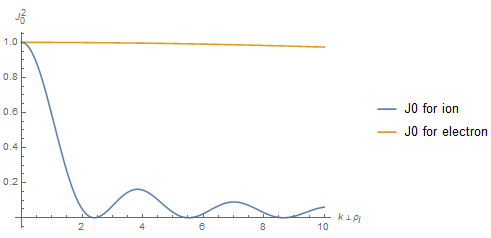
\includegraphics[width=0.9\textwidth]{Image/J0_1.PNG}
        \caption{plot of $J_0^2(k_\perp\rho_i)$ different species, small $k_\perp$}
        \label{fig:J0_1}
\end{figure}

\begin{figure}[h] \centering
        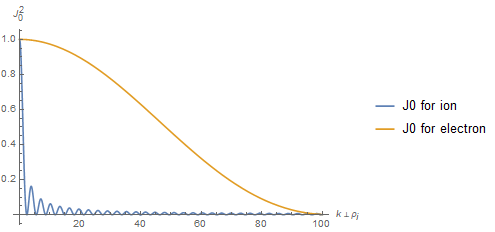
\includegraphics[width=0.9\textwidth]{Image/J0_2.PNG}
        \caption{plot of $J_0^2(k_\perp\rho_i)$ different species, large $k_\perp$}
        \label{fig:J0_2}
\end{figure}








\section{Mode induction}

All the modes are driven by the pressure gradient($\omega_{*}^{tot}$).


Perturbation of magnetic field induces electromagnetic mode - MTM. 

Let's first talk about the source of the perturbation. As the electrons and ions move (roughly) along the field line. Moving charge induces a magnetic field. From the large scale, the total magnetic perturbation should be small due to quasi-neutrality. 

\section{Mode stabilization}

Landau damping, magnetic shear suppression and $E\times B$ shear suppression 

\section{Transport}

The equation of the kinetic equation can be expressed in the following way. 

\begin{equation}
    \frac{\partial f}{\partial t} = \mathcal{L}[f]+\mathcal{N}[f,f]
\end{equation}

Where $\mathcal{L}[f]$ is the linear term and $\mathcal{N}[f,f]$ is the nonlinear term. 

Recall in linear theory we have 
\begin{equation}
    \frac{\partial f}{\partial t} = \mathcal{L}[f]
\end{equation}

Where $ \frac{\partial f}{\partial t} =\gamma f$, 
With the assumption of $\mathcal{L}[f] \approx \gamma f$ 

One can express the nonlinear term in the following way: 

\begin{equation}
    \mathcal{N}[f,f] = \sum_{k'} \left(k_x'k_y-k_xk_y'\right)\phi_{k'} f_{k,k'}
\end{equation}
$\mathcal{N}[f,f] \approx -\overline{k^2_\perp} f \phi$ for sure a 

At the saturation level, $\frac{\partial f}{\partial t} = 0$

Therefore $\chi \propto \phi \approx \frac{\gamma}{\overline{k^2_\perp}}$

Recall from

\begin{equation}
    Q=n\chi \nabla T
\end{equation}

Taking magnetic instabilities into account, we have $\chi \propto \phi+v_{||}A_{||} $

Qusailinear magnetic transport will be 

\begin{eqnarray}
    \int k_y \chi v^2 f dv\\
    =\int k_y \phi v^2 f dv + 
      \int k_y v_{||}A_{||} v^2 f dv\\
    =v_{E\times B} \delta P
    +\delta B_x q_{|| e}
\end{eqnarray}

The flaw of this model is that, linear term only considers the on mode. 

\section{Parity}

Kinetic instibilities and MHD type instabilities. For kinetic instabilities, the distribution depends on frequncy, hence the plasma with different velocity responds to different frequency. 

\textbf{Tearing parity and Ballooning parity are two eigen-solution to a $2_{nd}$ order differential equation.} Tearing being odd in $\phi$ and Ballooning being even in $\phi$. From the equation 33-39 of \cite{tearing_parity}, the mathematical aspect of the parity has been illustrated. As we know, any function can be expressed in one even function add another odd function. The even and odd function will represent different type of instabilities with different physics

In general, the differential equations can be expressed as:

\begin{eqnarray}
    \mathcal{L}(x) f(x)=0 \\
    \left[\mathcal{L}_{even}(x)+\mathcal{L}_{odd}(x)\right]f(x)=0 
    \label{eq:lxfx}
\end{eqnarray}

Where the $\mathcal{L}(x)$ is a linear operator, $\mathcal{L}(x)$ has a odd and even part $\mathcal{L}(x)=\mathcal{L}_{even}(-x)-\mathcal{L}_{odd}(-x)$. So the we have

\begin{equation}
    \left[\mathcal{L}_{even}(-x)-\mathcal{L}_{odd}(-x)\right]f(x)=0
\end{equation}

Equivalently, changing $x$ to $-x$

\begin{equation}
    \left[\mathcal{L}_{even}(x)-\mathcal{L}_{odd}(x)\right]f(-x)=0 
    \label{eq:lxf-x}
\end{equation}

Combine Equation \ref{eq:lxfx} and Equation \ref{eq:lxf-x}. Then we will have,

\begin{eqnarray}
    \mathcal{L}_{even}(x) \left[\frac{f(x) + f(-x)}{2}\right]=0\\
    \mathcal{L}_{odd}(x)  \left[\frac{f(x) - f(-x)}{2}\right]=0
\end{eqnarray}

Where $\left[\frac{f(x) + f(-x)}{2}\right]$ is a general expression of even function. On the other hand, $\left[\frac{f(x) - f(-x)}{2}\right]$ is odd. 

For two coupled differential equations

\begin{eqnarray}
    \mathcal{L}_1(x) \phi(x)=g(x)\psi(x)\\
    \mathcal{L}_2(x) \psi(x)=h(x)\phi(x)
\end{eqnarray}

If the $g(x)$ and $h(x)$ are odd, meanwhile $\mathcal{L}_1$ and $\mathcal{L}_2$ are even. Similar to previous case

\begin{eqnarray}
    \mathcal{L}_1(x) \phi(-x)=-g(x)\psi(-x)\\
    \mathcal{L}_2(x) \psi(-x)=-h(x)\phi(-x)
\end{eqnarray}

If the $\phi(x)$ is even

\begin{eqnarray}
    \mathcal{L}_1(x) \phi(x)=-g(x)\psi(-x)\\
    \mathcal{L}_2(x) \psi(-x)=-h(x)\phi(x)
\end{eqnarray}

Then $\psi(s)$ has to be odd. 

\begin{eqnarray}
    \mathcal{L}_1(x) \phi(x)=g(x)\psi(x)\\
    \mathcal{L}_2(x) \psi(x)=h(x)\phi(x)
\end{eqnarray}

Similarly, we will have the case where $\phi(x)$ is odd and $\psi(x)$ is even. 

From \cite{parity} Figure \ref{fig:parity} 

\begin{figure}[h] \centering
        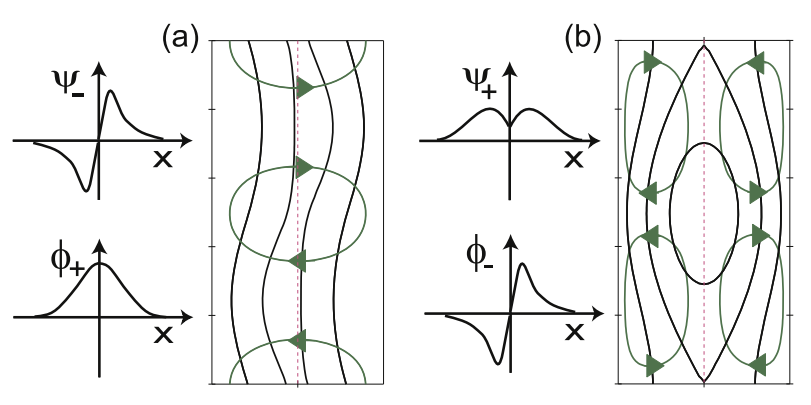
\includegraphics[width=1\textwidth]{Image/Parity.png}
        \caption{Figure7 from \cite{parity}. Electrostatic potential $\phi$ and perturbed magnetic flux $\psi$ profiles of (a) twisting parity mode $\left(\phi_{+}, \psi_{-}\right)$ and (b) tearing parity $\operatorname{mode}\left(\phi_{-}, \psi_{+}\right)$ in a slab plasma.}
        \label{fig:parity}
\end{figure}


\subsection{Ballooning parity}
\subsection{Tearing parity}

The $A_{||}$ being even around rational surface will provide the structure like olive. 

\chapter{Ion Temperature Gradient Mode}
Recall from Equation \ref{eq:linear} and Equation \ref{eq:rho=0}

\begin{equation}
    \delta f_s(\textbf{v},\textbf{X},t)=-\frac{q_s\phi}{T_s}F_{0,s}+
    \frac{\omega -\omega_*^{tot} 
    }{\omega -\omega_D 
    - k_{||}v_{||}-i\nu(h_s)}\left(\frac{q_s\phi}{T_s}-\frac{q_sA_{||}v_{||}}{cT_s}\right)J_0^2(k_\perp\rho_s)F_{0,s}
\end{equation}

\begin{equation}
\rho_{tot}=\sum_{s} q_s\int d\textbf{v} \delta f=0
\end{equation}

With two Equations above, with $A_{||}=0$ and $\delta f= h_i + \frac{q_e \phi}{T_e} F_{0,e}+ \frac{q_i \phi}{T_i} F_{0,i}$

\begin{equation}
\begin{aligned}
\rho_{tot}{}&=\sum_{s} q_s\int d\textbf{v} \delta f\\
&=\int d\textbf{v} \left(q_ih_i(\textbf{v},\textbf{X},t) + \frac{q_e^2 \phi}{T_e} F_{0,e}+ \frac{q_i^2 \phi}{T_i} F_{0,i}\right)\\
&=\int d\textbf{v} \left[q_i
\frac{\omega -\omega_*^{tot} 
    }{\omega -\omega_D 
    - k_{||}v_{||}-i\nu(h_s)}\frac{q_i\phi}{T_s}J_0^2(k_\perp\rho_i)F_{0,i}
+ \frac{q_e^2 \phi}{T_e} F_{0,e}+ \frac{q_i^2 \phi}{T_i} F_{0,i}\right]\\
\end{aligned}
\end{equation}

Since $\int F_{0,s}d\textbf{v}=n_s$ and $\rho_{tot}=0$

\begin{equation}
   \frac{n_e}{T_e} + \frac{n_i }{T_i}+\frac{q_i^2}{q_e^2} \frac{1}{T_i} \int d\textbf{v} \left[
\frac{\omega -\omega_*^{tot} 
    }{\omega -\omega_D 
    - k_{||}v_{||}-i\nu(h_s)}J_0^2(k_\perp\rho_i)F_{0,i}
 \right]=0
\label{eq:ITG}
\end{equation}

For the future calculation, $q_i=e$, $n_i=n_e= $ will be assumed, therefore 

\begin{equation}
   \frac{1}{T_e} + \frac{1}{T_i}+\frac{1}{T_i} \int d\textbf{v} \left[
\frac{\omega -\omega_*^{tot} 
    }{\omega -\omega_D 
    - k_{||}v_{||}-i\nu(h_s)}J_0^2(k_\perp\rho_i)F_{0,i}
 \right]=0
\end{equation}

Reall $\omega_{*}^{T o t}=\omega_{* n}+\left(-\frac{3}{2}+\frac{v_{\perp}^{2}+v_{ \|}^{2}}{2 v_{t h}^{2}}\right) \omega_{* T}$ and $\rho_s=\frac{m_sv_\perp}{q_sB}$

\begin{equation}
\begin{aligned}
   \frac{1}{T_e} + \frac{1}{T_i}+\frac{1}{T_i} 
   \int d\textbf{v} \left[
\frac{1 
    }{1 -\frac{\omega_D }{\omega}
    - \frac{k_{||}v_{||}}{\omega}-\frac{i\nu(h_s)}{\omega}}J_0^2(k_\perp\rho_i)F_{0,i}
 \right]
 \\
 +\frac{1}{T_i}\frac{\omega_{*n}}{\omega} 
   \int d\textbf{v} \left[
\frac{1 
    }{1 -\frac{\omega_D }{\omega}
    - \frac{k_{||}v_{||}}{\omega}-\frac{i\nu(h_s)}{\omega}}J_0^2(k_\perp\rho_i)F_{0,i}
 \right]
 \\
  -\frac{3}{2}\frac{1}{T_i} \frac{\omega_{*T} }{\omega}
   \int d\textbf{v} \left[
\frac{1 
    }{1 -\frac{\omega_D }{\omega}
    - \frac{k_{||}v_{||}}{\omega}-\frac{i\nu(h_s)}{\omega}}J_0^2(k_\perp\rho_i)F_{0,i}
 \right]
  \\
  +\frac{1}{T_i} \frac{\omega_{*T} }{\omega}
   \int d\textbf{v} \left[
\frac{\frac{v_{\perp}^{2}+v_{ \|}^{2}}{2 v_{t h}^{2}} 
    }{1 -\frac{\omega_D }{\omega}
    - \frac{k_{||}v_{||}}{\omega}-\frac{i\nu(h_s)}{\omega}}J_0^2(k_\perp\rho_i)F_{0,i}
 \right]
 =0
 \end{aligned}
\end{equation}

Assume $A(\textbf{k},\omega, \omega_D ,\nu)=
\int d\textbf{v} \left[
\frac{1 
    }{1 -\frac{\omega_D }{\omega}
    - \frac{k_{||}v_{||}}{\omega}-\frac{i\nu(h_s)}{\omega}}J_0^2(k_\perp\rho_i)F_{0,i}
 \right]
$ and 
$B(\textbf{k},\omega, \omega_D,\nu)=
\int d\textbf{v} \left[
\frac{\frac{v_{\perp}^{2}+v_{ \|}^{2}}{2 v_{t h}^{2}}  
    }{1 -\frac{\omega_D }{\omega}
    - \frac{k_{||}v_{||}}{\omega}-\frac{i\nu(h_s)}{\omega}}J_0^2(k_\perp\rho_i)F_{0,i}
 \right]
$ , After some algebra:

\begin{equation}
    \frac{1}{T_e}+
    \frac{1}{T_i}+
    \frac{1}{T_i}A\left(1+\frac{\omega_{*n}}{\omega}-\frac{3}{2}\frac{\omega_{*T}}{\omega}\right)+\frac{1}{T_i} B\frac{\omega_{*T}}{\omega}=0
\end{equation}

\section{Analytical approach}

One can solve the equation using some approximation

Assume $\frac{\omega_{D}}{\omega} \ll 1$, $\frac{k_{||}v_{||}}{\omega} \ll 1$ and $\frac{\nu}{\omega} \ll 1$. 

Since $\frac{1}{1-x}=1+x$ for small x.

We have $A(\textbf{k},\omega, \omega_D ,\nu)=
\int d\textbf{v} \left[
1 +\frac{\omega_D }{\omega}
    + \frac{k_{||}v_{||}}{\omega}
    +\frac{i\nu(h_s)}{\omega}\right]
    J_0^2(k_\perp\rho_i)F_{0,i}$ 
    and 
    $B(\textbf{k},\omega, \omega_D ,\nu)=
\int d\textbf{v} 
\frac{v^2_{\perp}+v_{||}^2}{2v_{th}^2}
\left[
1 +\frac{\omega_D }{\omega}
    + \frac{k_{||}v_{||}}{\omega}+\frac{i\nu(h_s)}{\omega}\right]
    J_0^2(k_\perp\rho_i)F_{0,i}$.
    For simplicity, we define $A=\alpha_0+\frac{\alpha_1}{\omega}$, where $\alpha_0=\int d\textbf{v} 
    J_0^2(k_\perp\rho_i)F_{0,i}$ and\\
    $\frac{\alpha_1}{\omega}=
    \int d\textbf{v} \left[
\frac{\omega_D }{\omega}
    + \frac{k_{||}v_{||}}{\omega}
    +\frac{i\nu(h_s)}{\omega}\right]
    J_0^2(k_\perp\rho_i)F_{0,i}$. Similar for B: $B=\beta_0+\frac{\beta_1}{\omega}$, 
    where 
    $\beta_0=\int d\textbf{v} \frac{v^2_{\perp}+v_{||}^2}{2v_{th}^2}
    J_0^2(k_\perp\rho_i)F_{0,i}$ and\\
    $\frac{\beta_1}{\omega}=
    \int d\textbf{v} \frac{v^2_{\perp}+v_{||}^2}{2v_{th}^2}
    \left[
\frac{\omega_D }{\omega}
    + \frac{k_{||}v_{||}}{\omega}
    +\frac{i\nu(h_s)}{\omega}\right]
    J_0^2(k_\perp\rho_i)F_{0,i}$
    
    Only take the $0_{th}$ order and the first order terms, then the dispersion relation becomes, 
    
    \begin{eqnarray}
        \begin{aligned}
    \frac{1}{T_e}+
    \frac{1}{T_i}+
    \frac{1}{T_i}(\alpha_0+\frac{\alpha_1}{\omega})\left(1+\frac{\omega_{*n}}{\omega}-\frac{3}{2}\frac{\omega_{*T}}{\omega}\right)+\frac{1}{T_i}(\beta_0+\frac{\beta_1}{\omega})\frac{\omega_{*T}}{\omega}{}&=0
    \end{aligned}
    \end{eqnarray}
    
    Now express it into 1, $\frac{1}{\omega}$, $\frac{1}{\omega^2}$. 
    \begin{eqnarray}
        \begin{aligned}
    \left(
    \frac{1}{T_e}+
    \frac{1}{T_i}+
    \frac{\alpha_0}{ T_i}
    \right)+
    \frac{1}{\omega}
    \left[
    \frac{\alpha_0\omega_{*n}}{T_i}-
    \frac{3\alpha_0\omega_{*T}}{2 T_i}+
    \frac{\alpha_1}{T_i}+
    \frac{\beta_0\omega_{*T}}{T_i}
    \right]\\
    +
    \frac{1}{\omega^2}
    \left(
    \frac{\alpha_1\omega_{*n}}{ T_i}-
    \frac{3\alpha_1\omega_{*T}}{2 T_i}+
    \frac{\beta_1\omega_{*T}}{T_i}
    \right)
    &=0
    \end{aligned}
    \end{eqnarray}
    
    Then we arrive to a neat expression
    
    \begin{equation}
        a\omega^2+b\omega+c=0
    \end{equation}
    
    Where $a=\left(
    \frac{1}{T_e}+
    \frac{1}{T_i}+
    \frac{\alpha_0}{ T_i}
    \right)$,
    $b=\left[
    \frac{\alpha_0\omega_{*n}}{ T_i}-
    \frac{3\alpha_0\omega_{*T}}{2 T_i}+
    \frac{\alpha_1}{ T_i}+
    \frac{\beta_0\omega_{*T}}{T_i}
    \right]
    $,
    $c=
    \left(
    \frac{\alpha_1\omega_{*n}}{ T_i}-
    \frac{3\alpha_1\omega_{*T}}{2 T_i}+
    \frac{\beta_1\omega_{*T}}{T_i}
    \right)
    $
    
    The general solution will be 
    
    \begin{equation}
     \omega=\frac{-b \pm \sqrt{b^{2}-4 a c}}{2 a}
    \end{equation}
    
    \begin{eqnarray}
        \begin{aligned}
        \gamma{}&=Im[\omega]\\
        &=Im[\frac{\sqrt{b^2-4ac}}{2a}]
        \end{aligned}
    \end{eqnarray}
    
        
    
    One can further simplify the equation by making more assumptions,
    
    $(k_\perp\rho_i)\rightarrow 0$, $J_0^2(k_\perp\rho_i)\rightarrow 1$, therefore
    \begin{eqnarray}
        \begin{aligned} 
        \alpha_0{}&=\int d\textbf{v}     F_{0,i}\\
        &=\int^\infty_0 dv \int ^\pi_0 d\theta \int ^{2\pi}_0 d\phi v^2sin\theta (\frac{1}{2\pi})^{3/2}\frac{1}{v_{th}^3}e^{-\frac{v^2}{2v_{th}^2}}\\
        &=\int^\infty_0 ds \int ^\pi_0 d\theta s^2sin\theta (\frac{1}{2\pi})^{1/2}e^{-\frac{s^2}{2}}\\
        &=1
        \end{aligned}
    \end{eqnarray}
    and
    \begin{eqnarray}
        \begin{aligned} 
        \beta_0{}&=\int d\textbf{v} \frac{v^2_{\perp}+v_{||}^2}{2v_{th}^2} F_{0,i}\\
        &=\int^\infty_0 dv \int ^\pi_0 d\theta \int ^{2\pi}_0 d\phi v^2sin\theta (\frac{1}{2\pi})^{1/2}\frac{v^2}{2v_{th}^2}\frac{1}{v_{th}^3}e^{-\frac{v^2}{2v_{th}^2}}\\
        &=\int^\infty_0 ds (\frac{1}{2\pi})^{1/2}s^4e^{-\frac{s^2}{2}}\\
        &=\frac{3}{2}
        \end{aligned}
    \end{eqnarray}
    
    With $\omega_D=\omega_{D0}\left(\mathrm{v}_{ \|}^{2}+\mathrm{v}_{\perp}^{2} / 2\right) / \mathrm{v}_{t h}^{2}$, define $s=\frac{v}{v_{th}}$. $v_{th}=\sqrt{T_i/m_i}$ Recall $F_{0,s}(v)=\left(\frac{m_s}{2\pi T_s}\right)^{3/2}e^{-m_sv^2/2T_s}=(\frac{1}{2\pi})^{3/2}\frac{1}{v_{th}^3}e^{-\frac{v^2}{2v_{th}^2}}$, 
    
    Useful formula: $\int^\infty_0 x^ne^{-ax^2}=(\pi/2)^{1/2}(n-1)!!(2a)^{-\frac{n+1}{2}}$ for $n>0$ and even
    \begin{eqnarray}
        \begin{aligned}
        \alpha_1{}&=
    \int d\textbf{v} \left[\omega_D\left(\mathrm{v}_{ \|}^{2}+\mathrm{v}_{\perp}^{2} / 2\right) / \mathrm{v}_{t h}^{2}
    + k_{||}v_{||}
    +i\nu(h_s)\right]
    J_0^2(k_\perp\rho_i)F_{0,i}\\
    &=\int^\infty_0dv \int^{\pi}_0 d\theta s^2sin(\theta) [\omega_D s^2(1-\frac{1}{2}sin^2\theta)
    + k_{||}s v_{th} cos\theta\\
    &\ \ +i\nu(h_s)]
    J_0^2(k_\perp\rho_i)(\frac{1}{2\pi})^{1/2}e^{-\frac{s^2}{2}}\\
    &= 2\omega_{D0}+k_{||}v_{th}\cdot 0 +i\nu
        \end{aligned}
    \end{eqnarray}
    
    Similarly,
        \begin{eqnarray}
        \begin{aligned}
        \beta_1{}&=
    \int d\textbf{v} \frac{v^2_{\perp}+v_{||}^2}{2v_{th}^2}\left[\omega_D\left(\mathrm{v}_{ \|}^{2}+\mathrm{v}_{\perp}^{2} / 2\right) / \mathrm{v}_{t h}^{2}
    + k_{||}v_{||}
    +i\nu(h_s)\right]
    J_0^2(k_\perp\rho_i)F_{0,i}\\
    &=\int^\infty_0dv \int^{\pi}_0 d\theta s^2\frac{s^2}{2} sin(\theta) [\omega_D s^2(1-\frac{1}{2}sin^2\theta)
    + k_{||}s v_{th} cos\theta\\
    &\ \ +i\nu(h_s)]
    J_0^2(k_\perp\rho_i)(\frac{1}{2\pi})^{1/2}\frac{1}{v_{th}}e^{-\frac{s^2}{2}}\\
    &= 5\omega_{D0}+k_{||}v_{th}\cdot 0 +\frac{i3\nu}{2}
        \end{aligned}
    \end{eqnarray}
    
    Assume $\nu=0$, plug everything to $b^2-4ac$, then we have:
    
    \begin{equation}
        b^2-4ac=\frac{T_e \left[4 \omega_{D0}^2-4 \omega_{D0} (3  \omega_{*n}+4  \omega_{*T})+ \omega_{*n}^2\right]-8 T_i \omega_{D0} ( \omega_{*n}+ \omega_{*T})}{T_e T_i^2}
    \end{equation}
    
    The equation is still to complicated. Since $\omega_{*n}\gg \omega_{D0}$, $\omega_{*T}\gg \omega_{D0}$, if we assume $\omega_{*n}=0$ and take the first order, then we will have $\alpha_1=\beta_1=0$. with $\alpha_0=0 $ and $\beta_0=\frac{3}{4} $ Then we will have a simple expression for real frequency and growth.
    
    \begin{equation}
        \gamma=\pm \sqrt{\frac{2T_e\omega_{D0}\omega_{*T}}{2T_e+T_i}}
    \end{equation}
    
    
    \begin{equation}
        \omega=\frac{-\omega_{*n}}{2(\frac{T_i}{T_e}+2)}
    \end{equation}
    
    
    


\section{Numerical approach}

One can also solve for the frequency and growth rate numerically. 

Solve for $\omega$:

\begin{equation}
    \omega = \frac{A(\omega_{*n}-\frac{3}{2}\omega_{*T})+B\omega_{*T}}{\frac{ T_e}{T_e+T_i}-A}
\end{equation}

Solve the equation using spherical coordinates $v_{||}=vcos\theta$, $v_{\perp}=vsin\theta$, $F_{0,s}(v)=\left(\frac{m_s}{2\pi T_s}\right)^{3/2}e^{-m_sv^2/2T_s}$

\begin{equation}
    \begin{aligned}
    A(\textbf{k},\omega, \omega_D ,\nu){}&=
\int d\textbf{v} \left[
\frac{1 
    }{1 -\frac{\omega_D }{\omega}
    - \frac{k_{||}v_{||}}{\omega}-\frac{i\nu[h_i]}{\omega}}J_0^2(k_\perp\rho_i)\left(\frac{m_i}{2\pi T_i}\right)^{3/2}e^{-m_sv^2/2T_i}
 \right]\\
 &=
2\pi \int^\pi_0 d\theta \int ^\infty _0 dv \left[
\frac{1 
    }{1 -\frac{\omega_D }{\omega}
    - \frac{k_{||}s_iv_{i,th}cos\theta}{\omega}-\frac{i\nu[h_i]}{\omega}}J_0^2(k_\perp\rho_i)\left(\frac{v^2_{i,th}}{2\pi T_i}\right)^{3/2}e^{-s_i^2
    }
 \right]
    \end{aligned}
\end{equation}

Where $s_i=\frac{v}{v_{th,i}}$,Similarly

\begin{equation}
    \begin{aligned}
    B(\textbf{k},\omega, \omega_D,\nu){}&=
\int d\textbf{v} \left[
\frac{\frac{v_{\perp}^{2}+v_{ \|}^{2}}{2 v_{t h}^{2}}  
    }{1 -\frac{\omega_D }{\omega}
    - \frac{k_{||}v_{||}}{\omega}-\frac{i\nu(h_s)}{\omega}}J_0^2(k_\perp\rho_i)\left(\frac{m_i}{2\pi T_i}\right)^{3/2}e^{-m_sv^2/2T_i}
 \right]\\
 &=
2\pi \int^\pi_0 d\theta \int ^\infty _0 dv \left[
\frac{s_i^{2}  
    }{2\left(1 -\frac{\omega_D }{\omega}
    - \frac{k_{||}vcos\theta}{\omega}-\frac{i\nu(h_s)}{\omega}\right)}J_0^2(k_\perp\rho_i)F_{0,i}
 \right]
    \end{aligned}
\end{equation}


\section{Parameter}
ITG
\begin{eqnarray}
    k_y\rho_i 0.1~0.5
\end{eqnarray}

\section{$k_{||}v_{||,i}, \omega_{D,i} << \omega$ with low-$k_{\perp}$ Limit}
\begin{eqnarray}
    \omega_{D,i}=\vec{k}\vec{v}_D=k_{y}\frac{v_{\perp}^2/2+v_{\parallel}^2}{R\Omega}\\
    \omega_{D,i}=k_y \frac{v_{\perp}^2/2+v_{\parallel}^2}{v_{\perp}}\\
    \frac{k_{\perp} v_{||}^2}{v_{\perp}}<<\omega\\
        (\frac{k_{||}}{k_\perp})^{-1} (\frac{v_{||}}{v_{\perp}})(k_{||} v_{||})<<\omega\\
    k_{||}v_{||}<<\omega
\end{eqnarray}

The dispersion relationship is 
\begin{eqnarray}
    \omega^3-\omega_{}
\end{eqnarray}

\chapter{Electron Temperature Gradient Mode}
The perturbed term for ETG is 
$\delta f= h_e + \frac{q_e \phi}{T_e} F_{0,e}+ \frac{q_i \phi}{T_i} F_{0,i}$.
Therefore we will will arrive with exact same answer as ITG with subscribe "i" and "e" swapped. 



\chapter{Trapped Electron Mode}
TEM is in between ITG and ETG. 

\chapter{Micro Tearing Mode}
\label{ch:MTM}



Let's first consider $k_{||}v_{||}<< \nu<< \omega$

\begin{eqnarray}
     \frac{B}{A}=\frac{ \int ^{\infty} _{0}   dv \frac{v^4(\frac{v^2}{2v^2_{th}}-3/2) }{1-i\frac{\nu_0\cdot v_{th}^3}{\omega v^3}} e^{-m_sv^2/2T_s}
     }{\int ^{\infty} _{0}   dv \frac{v^4}{1-i\frac{\nu_0\cdot v_{th}^3}{\omega v^3}} e^{-m_sv^2/2T_s}
     }
\end{eqnarray}
There are $\omega$ on both sides, it is hard to solve for analytically. But one can get solution with ease when we take two extreme cases. 
\begin{enumerate}
    \item For $\frac{\nu_0}{\omega}\longrightarrow 0$
    \begin{eqnarray}
         \frac{B}{A}=\frac{ \int ^{\infty} _{0}   dv \cdot v^5(\frac{v^2}{2v^2_{th}}-3/2) (1+i\frac{\nu_0\cdot v_{th}^3}{\omega v^3}) e^{-m_sv^2/2T_s}
     }{\int ^{\infty} _{0}   dv\cdot v^5 (1+i\frac{\nu_0\cdot v_{th}^3}{\omega v^3}) e^{-m_sv^2/2T_s}
     }\\
     \frac{B}{A}=\frac{2 m v_{th}^2}{3 (T - m v_{th}^2)}
    \end{eqnarray}
    \item For $\frac{\nu_0}{\omega}\longrightarrow \infty$
    \begin{eqnarray}
         \frac{B}{A}=\frac{ \int ^{\infty} _{0}   dv \cdot v^7(\frac{v^2}{2v^2_{th}}-3/2) e^{-m_sv^2/2T_s}
     }{\int ^{\infty} _{0}   dv\cdot v^7 e^{-m_sv^2/2T_s}
     }\\
     \frac{B}{A}=\frac{4 m v_{th}^2}{3 (3 T - 2 m v_{th}^2)}
    \end{eqnarray}
\end{enumerate}

Now let's take $k_{||}v_{||}$ into consideration. The analysical solution is almost impossible. We will do it purely numerically, Recall Equation \ref{eq:omega}. We have: 

\begin{eqnarray}
     \frac{B}{A}=\frac{\int^{\pi}_{0}d\theta \int ^{\infty} _{0}   dv \frac{v^4(\frac{v^2}{2v^2_{th}}-3/2) sin\theta cos^2\theta}{1-\frac{k_{||}v cos(\theta)}{\omega}-i\frac{\nu_0\cdot v_{th}^3}{\omega v^3}} e^{-m_sv^2/2T_s}
     }{\int^{\pi}_{0}d\theta \int ^{\infty} _{0}   dv \frac{v^4 sin\theta cos^2\theta}{1-\frac{k_{||}v cos(\theta)}{\omega}-i\frac{\nu_0\cdot v_{th}^3}{\omega v^3}} e^{-m_sv^2/2T_s}
     }
\end{eqnarray}
Solve for $\omega$ and substitute $s=\frac{v}{v_{th}}$,one can get
\begin{eqnarray}
     \omega=\omega_{*n}+\frac{B}{A}\omega_{*T}\\
     \frac{B}{A}=\frac{\int^{\pi}_{0}d\theta \int ^{\infty} _{0}   dv \frac{s^4(\frac{s^2}{2}-3/2) sin\theta cos^2\theta}{1-\frac{k_{||}s\cdot v_{th} cos(\theta)}{\omega}-i\frac{\nu_0 }{\omega s^3}} e^{-s^2/2}
     }{\int^{\pi}_{0}d\theta \int ^{\infty} _{0}   dv \frac{s^4 sin\theta cos^2\theta}{1-\frac{k_{||}s\cdot v_{th} cos(\theta)}{\omega}-i\frac{\nu_0 }{\omega s^3}} e^{-s^2/2}
     }
     \label{eq:B/A}
\end{eqnarray}

And the $\frac{B}{A}$ only depends on the two following to quantities: $\frac{k_{||}v_{th}}{\omega}$, $\frac{\nu_0}{\omega}$.

Using the following number for calculation
\begin{eqnarray}
     \eta=\frac{\omega_{*T}}{\omega_{*n}}=1.5\\
     q=4\\
     T_e=0.4keV\ \ \ (in GENE)\\
     k_{||}=\frac{in}{R}(1-\frac{m}{nq})
     v_{th}=\\
     L_s=8m\\
     k_y=0.1\\
     kx=0\\
     k_{||}=k_y(GENE)/L_s=1/80 m^{-1}
\end{eqnarray}

\begin{eqnarray}
     \omega=\omega_{*n}(1+1.5\frac{B}{A})
\end{eqnarray}

One can calculate the it numerically using Mathematica. 

Here is the $k_{||}=0$ shown in Figure \ref{fig:k_0}

\begin{figure}[h] \centering
        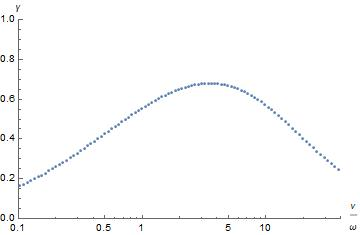
\includegraphics[width=1\textwidth]{Image/kpara=0.jpg}
        \caption{The growth rate of MTM with $k_{||}$=0}
        \label{fig:k_0}
\end{figure}


The Plot of growth rate with different k is shown in Figure \ref{fig:k_diff}

\begin{figure}[h] \centering
        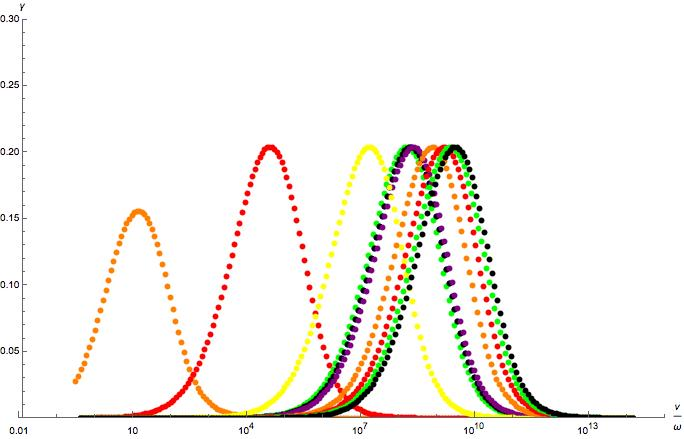
\includegraphics[width=1\textwidth]{Image/k_diff.jpeg}
        \caption{The growth rate of MTM with different k}
        \label{fig:k_diff}
\end{figure}

As Figure \ref{fig:k_peak} shown, the peak of the growth rate is sensitive of change of k near 0.

\begin{figure}[h] \centering
        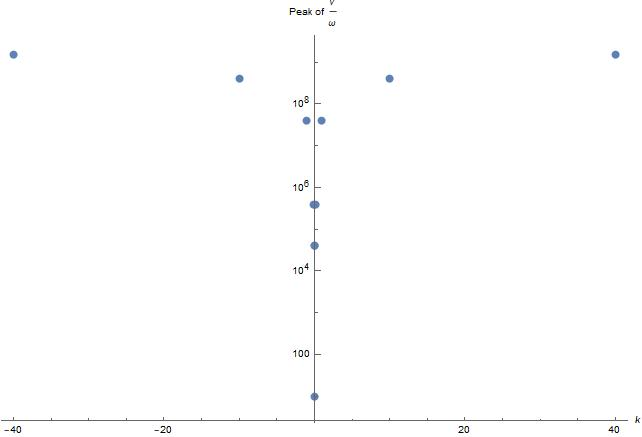
\includegraphics[width=1\textwidth]{Image/k_peak.jpg}
        \caption{The growth rate peak of MTM with changing k}
        \label{fig:k_peak}
\end{figure}


\chapter{MTM from Gladd, Drake}
\section{Eigenmode equation}
From the potential representation of the field:

\begin{equation}
    \begin{aligned}
    \textbf{B}=\nabla \times \textbf{A}_{||}\\
    \textbf{E}=-\nabla \phi -\frac{1}{c}\frac{\partial \textbf{A}_{||}}{\partial t}
    \end{aligned}
\end{equation}

With Ohm's Law and Maxwell's Equations

\begin{eqnarray}
    E_{||}=\frac{1}{\sigma_{||}}J_{||} \label{eq:ohm}\\
    \nabla \times \textbf{B} = 4\pi \textbf{J}
\end{eqnarray}

With some algebra (Assume $\hat{x}_{||}=\hat{z}$)
\begin{eqnarray}
\begin{aligned}
    (\nabla \times \textbf{B})_{||}{}&=[\nabla \times(\nabla \times \textbf{A}_{||}) ]_{||}\\
    &=[\nabla\cdot (\nabla\cdot A_{||}) - \nabla^2\textbf{A}_{||}]_{||}\\
    &=[(\hat{x}\frac{\partial }{\partial x}+
    \hat{y}\frac{\partial }{\partial y}+
    \hat{z}\frac{\partial }{\partial z}) (\frac{\partial }{\partial z} A_{||}) - (\frac{\partial^2 }{\partial x^2}+
    \frac{\partial^2 }{\partial y^2}+
    \frac{\partial^2 }{\partial z^2})\textbf{A}_{||}]_{||}\\
    &=(
   \frac{\partial }{\partial z}) (\frac{\partial }{\partial z} A_{||}) - (\frac{\partial^2 }{\partial x^2}+
    \frac{\partial^2 }{\partial y^2}+
    \frac{\partial^2 }{\partial z^2})\textbf{A}_{||}\\
    &=-(\frac{\partial^2 }{\partial x^2}+
    \frac{\partial^2 }{\partial y^2})\textbf{A}_{||}\\
    &=-\nabla_{\perp}^2 A_{||}
\end{aligned}
\end{eqnarray}

Assuming the time and spacial dependence: 
\begin{equation}
    \begin{aligned}
    \textbf{A}_{||}(\textbf{x},t)=\textbf{A}_{||}(x)exp(-i\omega t + ik_y y +ik_{||}z)\\
    \phi(\textbf{x},t)=\phi(x)exp(-i\omega t + ik_y y +ik_{||}z)
    \end{aligned}
\end{equation}

Plug into Equation \ref{eq:ohm}, 

\begin{eqnarray}
(\frac{\partial^2 }{\partial x^2}-k_y^2)A_{||}=-\frac{4\pi}{c}\sigma_{||}(x)E_{||}
\end{eqnarray}

Where $\sigma(x)=\int\frac{\omega-\omega_*}{\omega - k_{||}v_{||}-i\nu}\frac{cq_sF_{0,s}}{T_s}v_{||}^2dv$. If we goes to the high frequency region, we have $\sigma=\frac{1}{\lambda_s^2}$, where $\lambda_s$ is the skin depth. 

Now, let's do the some approximation about Equation \ref{eq:A2}. Since $k_{||}=k_y\frac{x}{L_s}$ and $x\rightarrow 0$, therefore one can do Taylor expansion around x=0:

\begin{eqnarray}
     \sigma(x)= \sigma(0) +\frac{x^2}{2}\sigma''(0)+ O(x^4)
\end{eqnarray}

Plug it back into the Equation \ref{eq:A2}, then we have:

\begin{eqnarray}
     (\frac{\partial^2 }{\partial x^2}-k_y^2)A_{||}\approx (\sigma(0) +\frac{x^2}{2}\sigma''(0)) \textbf{A}_{||}
     \label{eq:MTM_eigen}
\end{eqnarray}

Recall the equation resemble the equation of Harmonic Oscillator in Quantum Mechanics, \cite{QM}\cite{formula}

The equation of Harmonic Oscillator in Quantum Mechanics,

\begin{equation}
-\frac{\hbar^{2}}{2 m} \frac{\partial^{2} \psi_{n}}{\partial x^{2}}+\frac{1}{2} m \omega^{2} x^{2} \psi_{n}=E_{n} \psi_{n}
\end{equation}

The solution to that is 

\begin{equation}
\begin{array}{l}{\psi_{n}=\frac{H_{n}(x / a) \exp \left[-x^{2} /\left(2 a^{2}\right)\right]}{\left(n ! 2^{n} a \pi^{1 / 2}\right)^{1 / 2}}} \\ {\text { where } a=\left(\frac{\hbar}{m \omega}\right)^{1 / 2}}\end{array}
\end{equation}

Where $H_n$ is Hermite polynomials

\begin{equation}
\begin{array}{ll} & {H_{0}(y)=1, \quad H_{1}(y)=2 y, \quad H_{2}(y)=4 y^{2}-2...} \\  & {H_{n+1}(y)=2 y H_{n}(y)-2 n H_{n-1}(y)}\end{array}
\end{equation}

Compared with Equation \ref{eq:MTM_eigen}, 

\begin{eqnarray}
     (\frac{\partial^2 }{\partial x^2}-\frac{\sigma''(0)}{2}x^2)A_{||}\approx (\sigma(0)+k_y^2) \textbf{A}_{||}
\end{eqnarray}

Then we have following system of equations for normalization

\begin{equation}
    \begin{aligned}
    \frac{m^2\omega^2}{\hbar^2}=\frac{\sigma''(0)}{2}\\
    \frac{2mE_n}{\hbar^2}=\sigma(0)+k_y^2
    \end{aligned}
\end{equation}

Then we have the solution 

\begin{equation}
\begin{array}{l}{A_{||,n}=\frac{H_{n}(x / a) \exp \left[-x^{2} /\left(2 a^{2}\right)\right]}{\left(n ! 2^{n} a \pi^{1 / 2}\right)^{1 / 2}}} 
\\
{\text { where } a=\left(\frac{\sigma''(0)}{2}\right)^{-1 / 4}}
\end{array}
\end{equation}

Normalize $u=\frac{x}{a}$, then we have

\begin{equation}
    A_{||,n}=\left(\frac{\sigma''(0)}{2}\right)^{1 / 8}\frac{H_{n}(u) \exp \left(-u^{2} /2 \right)}{\left(n ! 2^{n}  \pi^{1 / 2}\right)^{1 / 2}}
\end{equation}

Figure \ref{fig:A_para} shows the first few eigenfunctions. 

\begin{figure}[h] \centering
        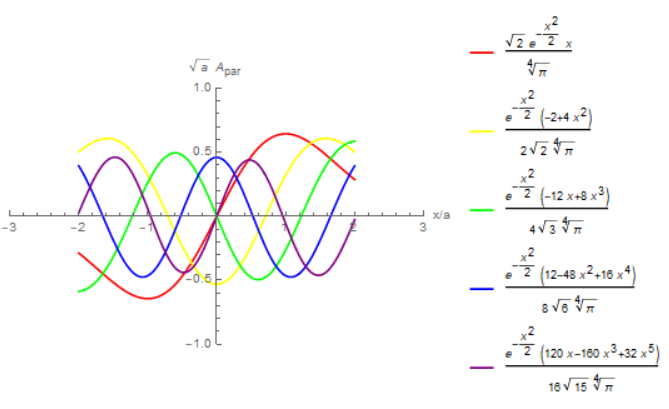
\includegraphics[width=0.8\textwidth]{Image/A_para.PNG}
        \caption{The growth rate peak of MTM with changing k}
        \label{fig:A_para}
\end{figure}



Integrate from both sides, we will be have

\begin{equation}
    \frac{dA}{dx}|^{x=l}_{x=-l} = \frac{4\pi}{c}\int ^{l}_{-l}dx j_{||}
\end{equation}

Since $\frac{1}{c^2}\frac{\partial ^2 }{\partial t^2} \sim k_{||}^2 \ll k^2$, then 

\begin{equation}
    \frac{d^2\textbf{A}_{||}}{dx^2} \approx \sigma(x) \textbf{A}_{||}
    \label{eq:A2}
\end{equation}

Where $\sigma(x)=\int\frac{\omega-\omega_*}{\omega - k_{||}v_{||}-i\nu}\frac{cq_sF_{0,s}}{T_s}v_{||}^2dv$

\subsection{Pertubation towards the exact solution}

From the quantized energy one can solve from quantuam mechanics: $E_n= (n+\frac{1}{2})\hbar \omega$, plug back into the transformation. 

\begin{equation}
    \sigma(0) +k_y^2 = (n+\frac{1}{2})\left[ 2 \sigma^{''}(0)\right]^{1/2}
\end{equation}





%\chapter{Micro Tearing Mode temp}
%
Magnetic perturbation induce MTM.\\

\begin{eqnarray}
    \nabla \times \vec{B} = \frac{4\pi }{c} \Vec{J}\\
    \nabla^2_{\perp} A_{||} \frac{4 \pi }{c} J_{||}
\end{eqnarray}

In cylinder geometry\\

\begin{eqnarray}
    \zeta =\frac{z}{2\pi R}\\
    \vec{B}=B_\zeta \vec{\zeta}+B_\theta \vec{\theta}\\
    \nabla =\frac{\partial }{\partial z} \hat{z}+ \frac{\hat{\theta}}{r} \frac{\partial }{\partial \theta}\\
    \vec{B} \nabla =i\frac{n}{R}(1-\frac{m}{n}q(r))
\end{eqnarray}

where $q=\frac{B_\zeta}{B_\theta}\frac{r}{R}$. 

The vlasov euqation 
\begin{eqnarray}
    \detal v_E= c \frac{\delta E \time B}{B^2}\\
    \frac{\partial \detla f}{\partial t}+v_{||} \frac{B \nabla \delta f}{|B|}+ v_{||}\frac{\detla B }{B} \nabla f_0\\
    (\omega - k_{||}v_{||})h+C[h]=\frac{qv_{||}}{T_s}\frac{A_{||}}{c} (\omega - \omega_*) f_{M}\\
    h=
    J_{||}=\int dv v_{||} \delta f\\
    \nabla \times \vec{B}=\vec{J}\\
    k_{||}=\frac{n}{R} (1- \frac{m}{n q(r)})\\
    q(r)=q(r_0)+(r+r_0)\frac{dq}{dr}\\
    q(r_0)=\frac{m}{n}\\
    k_{||}=\frac{n}{R}-\frac{mn}{Rr}\frac{1}{q^2}\frac{dq}{dr} \Delta r\\
    k_{||}= k_\theta \frac{\delta r}{L_s}\\
    L_s= \frac{qR}{\hat{s}}\\
    k_{||}v_{th}~ \omega \nu\\
    \frac{\Delta }{L_s} k_y v_e ~ \omega_*\\
    \omega = k_y\rho _s \frac{c_s}{L_p}\\
    L_p=\frac{1}{P_e}\frac{dp_e}{dr}\\
    c_s=\sqrt{\frac{T_e}{m_i}}\\
    \Delta r ~ \frac{L_s}{L_p}\rho_e
\end{eqnarray}

For core, $\frac{R}{L_p}~5-10$\\


GENE parameter
\begin{eqnarray}
    \hat{s}=1\\
    \alpha=q^2 R \frac{d\beta }{dr}\\
    \alpha=q^2 \frac{R}{L} \beta \\
    \beta = 2\beta_e \\
    \beta = 2q^2\frac{R}{L}\beta_e\\
    \alpha =3\\
    q=4\\
    \frac{R}{L}=40(core)
    \frac{R}{L}=160 (pedestal)\\
    \eta =1.5\\
    omn=64\\
    omt=96\\
    k_(Y,min)=k_{y,\rho}=0.1\\
    nxo=29
\end{eqnarray}

Finguer print for MTM
\begin{eqnarray}
    \frac{Q_{em}}{Q_{es}}>>1
\end{eqnarray}

\begin{equation}
    \frac{\partial f_s}{\partial t} + (v_{\parallel}\hat{b}+\textbf{v}_E+\textbf{v}_D)\cdot\nabla f_s + [q_s\textbf{E}\cdot(v_{\parallel}\hat{b}+\textbf{v}_D)]\frac{\partial f_s}{\partial \epsilon}=0
\label{eq:dke}
\end{equation}

\begin{eqnarray}
     i\omega f + i \textbf{k v} f + q \textbf{Ev} \frac{f}{\epsilon}=C
\end{eqnarray}
\begin{eqnarray}
     \textbf{v}=v_{||}\\
     (-i\omega +ik_{||}v_{||})\delta f=-\detal v \nabla F_0 -\frac{e}{m} \delta E_{||} \frac{df }{d x_{||}}\\
     \detal f =\frac{1}{-i\omega +ik_{||}v_{||}}(-\detal v \nabla F_0 -\frac{e}{m} \delta E_{||} \frac{df }{d x_{||}})\\
     <cos^2(\omega t)>=\frac{1}{2}\\
     \frac{d<f>}{dt}=\frac{\detal v \nabla <f>}{i\omega -k_{||}v_{||}}\\
     f~ e^{-n(\zeta -q \theta)}\\
     k_{\perp}-n\nabla(\zeta -q \theta)\\
     <\detal v \nabla f>=0\\
     <v \nabla \delta f>=0\\
     \int dx \longrightarrow \int dx \int dk \deta v_k e^{ikx}\delta v_k \int dk \delta f_{k'}\\
     \int dk i\frac{\delta v_k \delta v_k \nabla f_0}{\omega - k_{||}v_{||}}\\
     D=\int dk i\frac{\delta v_k \delta v_k }{\omega - k_{||}v_{||}}\\
\end{eqnarray}
Quasi linear\\
\begin{eqnarray}
     <\delta v \nabla \delta f>= \nabla <\delta v  \delta f>\\
     <\delta v  \delta f>=\Tau 
\end{eqnarray}
The dominant $\delta v$\\
\begin{eqnarray}
     MTM: \delta v=v_{||}; \delta n= v_{||}\frac{\delta B}{B}\\
     ITG: \delta v= v_{E\times B}=c\frac{c B \times \delta E}{B^2}\\
\end{eqnarray}
MTM particle flux
$\int dv \Tau = \int dv v_{||}\delta n \delta f$\\
$=\delta n \int dv v_{||}\delta f_{||}$\\
$=\frac{\delta B}{B} \delta j_{||}$\\
For heat flux
\begin{eqnarray}
     Q=\int dx \Tau \frac{1}{2} m v^2\\
     =\int v_{||}\frac{\delta B}{B} \delta f \frac{1}{2}mv^2\\
     =\frac{\delta B}{B}\int v_{||} \delta f \frac{1}{2}mv^2\\
     =\frac{\delta B}{B} \delta q_{||}\\
     =~(\frac{\delta B}{B})^2 \frac{\nabla f_0}{\omega}\nabla T\\
     D=~(\frac{\delta B}{B})^2 \nabla T\frac{v_{th}^2}{\omega}
\end{eqnarray}
Analysis the B field
\begin{eqnarray}
     \delta B=\nabla \times \delta A\\
     \nabla ^2 \delta A= \frac{k}{c} j_{||}
\end{eqnarray}
For test particle with distribution of g\\
\begin{eqnarray}
     \frac{dg}{dt} + \hat{n} \nabla g=0\\
     D~\frac{\delta n^2}{k_{||}}\\
     D_M~ \pi L_s(\frac{\delta B}{B})^2\\
     \frac{\delta B}{B}~10^{-4}
\end{eqnarray}

Both give us real number, which means we will have no instability on non-collisional or fully collisional limit. But there will be instablities arises in between which we will try to solve semi-analytically. 

We can do Tylor Expansion as following
\begin{eqnarray}
     \frac{1}{1-x}=\sum^\infty_{i=0} x^i\\
     A \propto \int ^\infty _0 \frac{v^8}{1+i\frac{v^3\omega}{\nu_0v_{th}^3}}dv\\
     %A \propto \int ^{\infty}_0 \sum^\infty_{n=0} (i\frac{\nu_0 v_{th}^3}{\omega})^nv^{5-3n}e^{-m_sv^2/2T_s}dv\\
     A \propto \int ^{\infty}_0 \sum^\infty_{n=0} (\frac{\omega}{i\nu_0 v_{th}^3})
     ^nv^{8+3n}e^{-m_sv^2/2T_s}dv\\
     B \propto \int ^{\infty}_0 \sum^\infty_{n=0} \frac{1}{2v^2_{th}}(\frac{\omega}{i\nu_0 v_{th}^3})
     ^nv^{10+3n}e^{-m_sv^2/2T_s}dv-\frac{3}{2}A
\end{eqnarray}

Recall the Gaussian integral, 
\begin{eqnarray}
     \int ^{\infty}_0 v^n\cdot e^{-mv^2/T}dv=\frac{1}{2} (\frac{m}{T})^{-\frac{1+n}{2}} \Gamma[\frac{n+1}{2}]\\
     A \propto \frac{1}{2} \sqrt{\frac{T}{m}} \sum^\infty_{n=0} (\frac{\omega}{i\nu_0 v_{th}^3}\sqrt{\frac{T}{m}})
     ^{n}   \Gamma[\frac{3n+9}{2}]\\
     B \propto \frac{1}{2} \frac{1}{2v^2_{th}} (\sqrt{\frac{T}{m}})^2 \sum^\infty_{n=0} (\frac{\omega}{i\nu_0 v_{th}^3}\sqrt{\frac{T}{m}})
     ^{n}   \Gamma[\frac{3n+11}{2}]
     -\frac{3}{2}A\\
     \frac{B}{A}=\frac{\sum^\infty_{n=0} \alpha
     ^{n}  \Gamma[\frac{3n+11}{2}]
     -\frac{3}{2}A
     }
     {2\sum^\infty_{n=0} \alpha
     ^{n}  \Gamma[\frac{3n+9}{2}]}\\
     \frac{B}{A}=\frac{\sum^\infty_{n=0} \alpha
     ^{n}  \Gamma[\frac{3n+11}{2}]
     }
     {2\sum^\infty_{n=0} \alpha
     ^{n}  \Gamma[\frac{3n+9}{2}]}-\frac{3}{2}
     %\\     \Gamma(z)=\int^\infty _0 x^{z-1}e^{-x}dx\\
     %\Gamma(z+1)=z\Gamma(z)
\end{eqnarray}

Where $\alpha=\frac{\omega}{i\nu_0 v_{th}^3}\sqrt{\frac{T}{m}}=\frac{\omega}{i\nu_0 v_{th}^2}$

Recall from Equation \ref{eq:omega}, we now have a better looking equation
\begin{eqnarray}
     i\nu_0v_{th}^2\alpha=\omega_{*n}+\frac{\sum^\infty_{n=0} \alpha
     ^{n}  \Gamma[\frac{3n+11}{2}]
     }
     {2\sum^\infty_{n=0} \alpha
     ^{n}  \Gamma[\frac{3n+9}{2}]}-\frac{3}{2}\omega_{*T}
     \label{eq:MTM-Z}
\end{eqnarray}

Recall $f\propto e^{-i\omega t} $, then we get $\omega=\omega_r+i\gamma$. We can divid the Equation \ref{eq:MTM-Z} into to part- real and imaginary

\begin{eqnarray}
     -\frac{\omega_r}{\nu_0v_{th}^2}=\omega_{*n}-\frac{3}{2}\omega_{*T}+Re(\frac{B}{A})\\
     \frac{\gamma}{\nu_0v_{th}^2}=Im(\frac{B}{A})
\end{eqnarray}


One can calculate the result numerically, the code for Mathematica is listed in Appendix. 

First, let's assume the right hand side $\omega$ is independent of left hand side's $\omega$. 

The plot is shown below as Figure \ref{fig:MTM} Figure \ref{fig:MTM2} Figure \ref{fig:MTM3} Figure \ref{fig:MTM4}. As we can see, with better and better $\alpha$ resolution. we ended up with a 

\begin{figure}[h] \centering
        \includegraphics[width=1\textwidth]{Image/MTM_growth.jpg}
        \caption{The growth rate of MTM}
        \label{fig:MTM}
\end{figure}

\begin{figure}[h] \centering
        \includegraphics[width=1\textwidth]{Image/MTM_growth2.jpg}
        \caption{The growth rate of MTM2}
        \label{fig:MTM2}
\end{figure}

\begin{figure}[h] \centering
        \includegraphics[width=1\textwidth]{Image/MTM_growth3.jpg}
        \caption{The growth rate of MTM3}
        \label{fig:MTM3}
\end{figure}

\begin{figure}[h] \centering
        \includegraphics[width=1\textwidth]{Image/MTM_growth3.jpg}
        \caption{The growth rate of MTM3}
        \label{fig:MTM3}
\end{figure}

\begin{figure}[h] \centering
        \includegraphics[width=1\textwidth]{Image/MTM_growth4.jpg}
        \caption{The growth rate of MTM4}
        \label{fig:MTM4}
\end{figure}

We can also solve the Equation \ref{eq:MTM-Z}, the Code is listed in the Appendix as well. 

\chapter{Tearing Mode temp}
With the knowledge of the Tearing mode, one can compare the Tearing mode with Micro Tearing mode (MTM).


From Ohm's Law 

\begin{equation}
    j_{||}=\sigma E = \sigma \frac{\gamma}{c} A_{||}
\end{equation}

Let's start from the quasi-neutrality argument.

\begin{eqnarray}
    \nabla J_{||} \approx \nabla \frac{\textbf{B}}{B} \textbf{J}=0\\
    \nabla (\frac{\textbf{B}_0+\delta \textbf{B}}{B})(\textbf{J}_0+\delta \textbf{J})=0
\end{eqnarray}

Recall 
\begin{eqnarray}
    \nabla(\textbf{J} \cdot \textbf{B}) \equiv \textbf{J} \times(\nabla \times \textbf{B})+(\textbf{J} \cdot \nabla) \textbf{B}+\textbf{B} \times(\nabla \times \textbf{J})+(\textbf{B} \cdot \nabla) \textbf{J}\\
    \nabla \times \mathbf{B}=\mu_{0}\left(\mathbf{J}+\varepsilon_{0} \frac{\partial \mathbf{E}}{\partial t}\right)\\
    \nabla \times \mathbf{E}=-\frac{\partial \mathbf{B}}{\partial t}
\end{eqnarray}

Then we only left with the dotted terms, 

\begin{equation}
    (\frac{\delta \textbf{B}}{B} \nabla )\textbf{J}_0+(\frac{\textbf{B}_0}{B} \nabla) \delta \textbf{J}=0
\end{equation}

Since $(\frac{\textbf{B}_0}{B} \nabla) = i \textbf{k}_{||}$

\begin{equation}
    (\frac{\delta \textbf{B}}{B} \nabla )\textbf{J}_0+ik_{||}\delta J_{||}=0
\end{equation}

From the Chapter \ref{ch:MTM}

\begin{eqnarray}
    (\frac{\partial^2}{\partial x ^2} -k_{y}^2)\delta A_{||}=-\frac{4\pi}{c} j_{||}
\end{eqnarray}

With Cylindrical coordinate and $k_y=\frac{m}{r}$ (From Equation \ref{eq:k_slab}) we have

\begin{eqnarray}
    \frac{1}{r}\frac{d}{dr}(r\frac{d \delta A_{||}}{dr}) -\frac{m^2}{r^2} \delta A_{||}=\frac{4\pi}{c} \delta j_{||}= \frac{4\pi}{c}\frac{\delta B_r}{B}\frac{\nabla j_0}{ik_{||}}\\
    \frac{1}{r}\frac{d}{dr}(r\frac{d \delta A_{||}}{dr}) -\frac{m^2}{r^2} \delta A_{||}=\frac{m}{r}\frac{\delta A_{||}}{k_{||}}\frac{\partial j_0}{\partial r} \frac{4\pi}{c}
\end{eqnarray}

Since $\delta B\approx \delta Ak_y$

\begin{eqnarray}
    \frac{1}{r}\frac{d}{dr}(r\frac{d \delta A_{||}}{dr}) -\frac{m^2}{r^2} \delta A_{||}=\frac{4\pi}{c} \delta j_{||}= \frac{4\pi}{c}\frac{\delta B_r}{B}\frac{\nabla j_0}{ik_{||}}\\
    \frac{1}{r}\frac{d}{dr}(r\frac{d \delta A_{||}}{dr}) -\frac{m^2}{r^2} \delta A_{||}=\frac{m}{r}\frac{\delta A_{||}}{k_{||}}\frac{\partial j_0}{\partial r} \frac{4\pi}{c}
\end{eqnarray}

Recall the common way to solve Boundary Condition problem in electrodynamics, 
$\delta A \propto r^{\pm m} $ is the solution to the problem. In order to make the function converge, we have 

\begin{eqnarray}
    \delta A = A_0 r^\alpha \ \ \ \ \ r>0\\
    \delta A = A_1 r^{-\alpha} \ \ \ \ \ r>r_{max}
\end{eqnarray}

To keep $\delta A$ analytical, we will determine the function in between using $\frac{dA}{dx}^{l}_{-l}$


\begin{eqnarray}
    j_{||} ~ \frac{1}{k_{||}}
\end{eqnarray}

By changing the profile of the current, one can avoid the tearing mode. 

However neoclassical tearing mode is hard to avoid. 

\section{Ohm's Law}

\begin{equation}
    \begin{aligned}
    \frac{1}{\sigma_{||}} j_{||}=\nabla_{||} \phi -\frac{1}{c}\frac{\partial A_{||}}{\partial t}=E_{||}\\
    \end{aligned}
\end{equation}

With Flux surface average $<Q>=\frac{1}{L}\int dl Q$, where $dl$ is following the field line. Since $<\nabla_{||} \phi>=\frac{\phi|^L_0}{L}=0$.

\begin{equation}
    \begin{aligned}
     \frac{1}{\sigma_{||}}<j_{||}>=-\frac{1}{c}<\frac{\partial A_{||}}{\partial t}>\\
     \delta A_{||}\approx -
    \end{aligned}
\end{equation}

$\Delta A=\Delta x j_{||}$

$\Delta x_{island} ~ A^{1/2}$

$\Delta x_{island} ~ t^{1/2}$ Which is Rutherford Theory



\chapter{Transport}
\section{H mode plasma}

\subsection{Higher core temperature}
For ITG-like modes, there is a critical gradient that once exceeded, the mode will be unstable. Therefore, at the steady state. we will have

\begin{equation}
    \frac{R}{L_{T}}=R \frac{1}{T}\frac{dT}{dr}
\end{equation}

Where $L_T$ is the critical gradient. The differential equation can solved easily which gives us. 

\begin{equation}
    T=T_0 e^{-(r-r_0)/L_T}
\end{equation}

For $r_0$ located at the top of the pedestal, we plug in $r=r_0$, then we have

\begin{equation}
    T=T_0
\end{equation}

Therefor the $T_0$ is the temperature of the top of the pedestal if $r=r_0$. 

From this point of view, The top of the pedestal will set the the temperature of the core. If the the pedestal is twice as high, then the core temperature will be roughly twice as high. 

\subsection{Confinement time}

Confinement time can be expressed as 

\begin{equation}
    \tau=\frac{E_{store}}{P_{input}}=\frac{3nT/2}{P} 
\end{equation}

For H-mode, if the core temperature is higher then the stored energy will higher, then the confinement time will longer. 

\subsection{Flat core profile}

For ITG-like mode, the transport is propotional to $T^{5/2}$. Therefore the profile will become more flat. 

\section{Diffusivity}

The definition of the particle diffusivity is (Fick's law on page 148) \cite{Chen}

\begin{eqnarray}
D_s = \Gamma_s(\frac{dn_s}{dx})^{-1}
\end{eqnarray}

Where $\Gamma_s$ is the flux of the species.

From the fluid equation of motion

\begin{equation}
    mn\frac{d\textbf{v}}{dt}=mn[\frac{\partial \textbf{v}}{\partial t}+(\textbf{v}\nabla)\textbf{v}]=\pm en \textbf{E}-\nabla p-mn\nu \textbf{v}
\end{equation}

For a steady state with small velocity, we can reduce the the equation into the following form: 

\begin{equation}
    \textbf{v}=\frac{1}{mn\nu}(\pm en \textbf{E}-\nabla p)
\end{equation}

With the definition of flux $\Gamma = n\textbf{v}$

We have

\begin{equation}
    \Gamma=\frac{1}{m\nu}(\pm en \textbf{E}-\nabla p)
\end{equation}

With the defination of the diffusivity $D=\frac{KT}{m\nu}$, and mobility $\mu=\frac{e}{m\nu}$, we arrive to the following equation.

\begin{equation}
    \Gamma =\pm \mu n \textbf{E} -D\nabla n 
\end{equation}



The definition of the heat diffusivity is

\begin{eqnarray}
\chi_s = (Q_s-\frac{3}{2}T_s\Gamma_s)(n_s \frac{dT_s}{dx})^{-1}
\end{eqnarray}

\subsection{Plasma parameter}

\begin{equation}
    g=\frac{1}{n_0\lambda_D}
\end{equation}

Where $\lambda_D=(\frac{kT}{8\pi n e^20})^{1/2}$

\section{Classical Transport}

\section{Neoclassical Transport}

Neoclassical transport is classical transport taking the effect of the device geometry. Effectively k=0 

\section{Anomalous Transport}

Anomalous transport is contributed by the turbulence. $k\neq 0$ 

\chapter{Ordering}
One can normalize the quantities to unit-less quantities for the purpose of numerical calculation and rough ordering estimate. This chapter will establish some ordering estimate for certain cases.

\section{DIII-D pedestal}

The calculation is based on a DIII-D H mode shot175823. Figure\ref{fig:ne} and Figure\ref{fig:Te}. 

\begin{figure}[h] \centering
        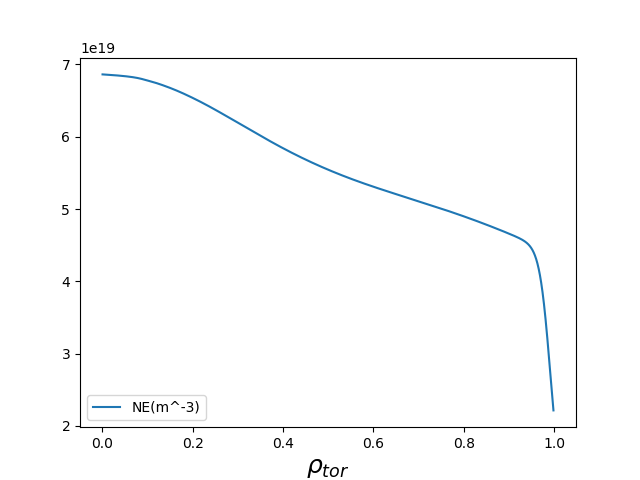
\includegraphics[width=1\textwidth]{Image/ne.png}
        \caption{The electron density}
        \label{fig:ne}
\end{figure}

\begin{figure}[h] \centering
        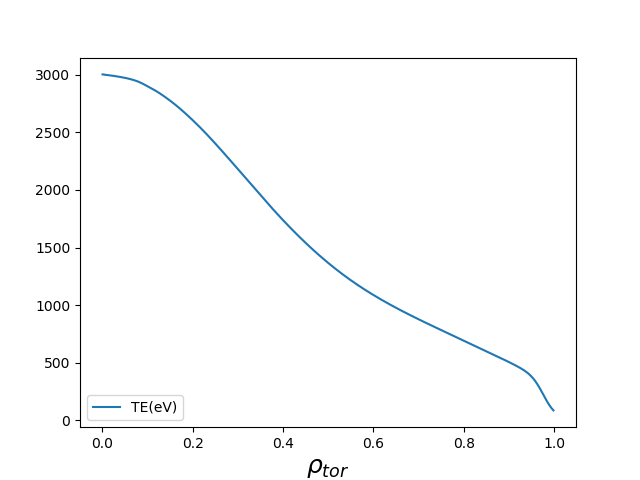
\includegraphics[width=1\textwidth]{Image/Te.png}
        \caption{The electron temperature}
        \label{fig:Te}
\end{figure}

At the mid pedastal(x/a=0.98) we have:\\
$a=0.67m$\\
$R=1.67m$\\
$B_0=2.2T$\\
$T_e=200eV$\\
$n_e=3.5\times 10^{19} /m^3$\\
$T_i=500eV$\\
$n_i=3.3\times 10^{19} /m^3$\\

People normalized frequency and growth rate in the unit of $c_s/a$

$c_s/a=\sqrt{\frac{\gamma k_B T}{M}}/a=282.9kHz$


Here are the unit-less quantities from a mid-pedestal of the DIII-D

$x=\frac{r}{a}=0.98$\\
$1/L_{n,e}=|\frac{1}{T_e}\frac{dT_e}{d x}|=25$\\
$1/L_{T,e}=|\frac{1}{T_e}\frac{dT_e}{d x}|=25$\\
$1/L_s=\frac{\hat{s}}{Rq}=\frac{1}{q}\frac{dq}{dx}=1$\\

\subsection{Typical waves}

$v_{th,s}=\sqrt{\frac{3 k_B T_s}{m_s}}$

Then $v_{th,i}=1.7\times 10^{5} m/s$

Diamagnetic Drift waves $\omega_{*e}=\frac{k_yT_e }{a L_n eB_0}=k_y*3.9*10^{23}$

Alfven wave $v_A=\frac{B_0}{\sqrt{4\pi m_in_i}}=1869m/s$

Cylotron frequency $\omega_c=\frac{e B_0}{m_i}=1.05\times 10^{8} rad/s$

Plamsa wave $\omega_p=\sqrt{\frac{n_0 e^2}{\epsilon_0 M}}=5.5\times 10^9 rad/s$

Gryoradius $\rho_i\approx \frac{v_{th,i}}{\omega_{c,i}}=1.6mm$






\chapter{General information of Fusion}
This Chapter is using Wesson's Tokamaks as a reference. 

\section{The reaction}

The most commonly used Thermal fusion fuel is Deuterium and tritium

\begin{equation}
_{1} \mathrm{D}^{2}+_{1} \mathrm{T}^{3} \rightarrow_{2} \mathrm{He}^{4}+_0\mathrm{n}^{1}
\end{equation}

This reaction generate 17.59MeV of energy. 

%With the concentration of 1 tritium atom per $10^{17}$ water molecules, 1 deuterium atom per 3200 water molecules, 1 ton of water can generate 0.94J of energy. 

To put it into perspective, 1oz of the tritium can produce $4.4GW\cdot h$ of energy. 

\section{Power Balance}

The reaction rate can be expressed in the following way, 

\begin{equation}
\mathcal{R}=\iint \sigma\left(v^{\prime} v^{\prime} f_{1}\left(v_{1}\right) f_{2}\left(v_{2}\right) \mathrm{d}^{3} v_{1} \mathrm{d}^{3} v_{2}\right.
\end{equation}

Where $\sigma$ is the cross section and $f(v_i)$ is the distribution. For most cases, Maxwellian distribution will relatively accurately describe the distribution inside of the reactor. 

Then the reaction rate can be rewriten in the following way: 

\begin{equation}
\begin{aligned} \mathcal{R}=n_{1} n_{2} & \frac{\left(m_{1} m_{2}\right)^{3 / 2}}{(2 \pi T)^{3}} \iint \exp \left(-\frac{m_{1}+m_{2}}{2 T}\left(\mathbf{V}+\frac{1}{2} \frac{m_{1}-m_{2}}{m_{1}+m_{2}} v^{\prime}\right)\right) \\ & \times \sigma\left(v^{\prime}\right) v^{\prime} \exp \left(-\frac{\mu v^{\prime}}{2 T}\right)^{2} \mathrm{d}^{3} v^{\prime} \mathbf{d}^{3} V \end{aligned}
\end{equation}

Where $$
\mathbf{V}=\frac{v_{1}+v_{2}}{2} \quad \text { and } \quad \mu=\frac{m_{1} m_{2}}{m_{1}+m_{2}}
$$

Integrate of V, then we got, 

\begin{equation}
\mathcal{R}=\left(\frac{8}{\pi}\right)^{1 / 2} n_{1} n_{2}\left(\frac{\mu}{T}\right)^{3 / 2} \frac{1}{m_{1}^{2}} \int \sigma(\varepsilon) \varepsilon \exp \left(-\frac{\mu \varepsilon}{m_{1} T}\right) \mathrm{d} \varepsilon
\end{equation}

Where \begin{equation}
\varepsilon=\frac{1}{2} m_{1} v^{\prime 2}
\end{equation}

The thermonuclear power can be expressed in the following way:

\begin{equation}
p_{\mathrm{T}_{0}}=\frac{1}{4} n^{2}<\sigma \nu> \mathcal{E}
\end{equation}

Where $<\sigma \nu>$ is the rate of reaction. 

\subsection{Power loss}

One can determine the power loss experimentally by supply the amount of energy $P_H+P_\alpha$ such that the system has the same energy density. 

\begin{equation}
P_{\mathrm{H}}+\frac{1}{4} \overline{n^{2}\langle\sigma v)} \varepsilon_{\alpha} V=\frac{3 \overline{n T}}{\tau_{\mathrm{E}}} V
\end{equation}

Where right hand side is the power loss. 

In order to sustain the fusion, $P_H <0$ is required. Therefore, we have the criteria 

\begin{equation}
n \tau_{\mathrm{E}}>\frac{12}{\langle\sigma v\rangle} \frac{T}{\varepsilon_{\alpha}}
\end{equation}

Plugin the physical number, we have a plot as Figure \ref{fig:ignition} shown. With T=30keV, we have


\begin{figure}[h] \centering
        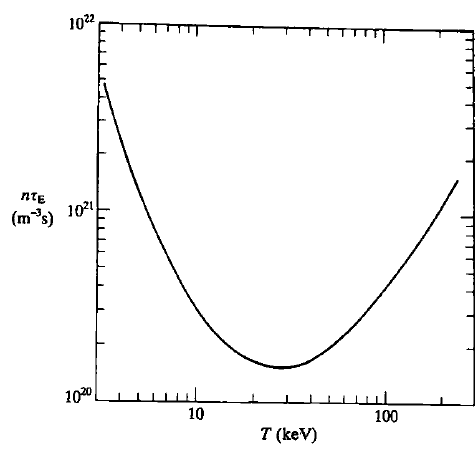
\includegraphics[width=0.4\textwidth]{Image/Ignition.png}
        \caption{$n\tau_E$ VS T}
        \label{fig:ignition}
\end{figure}

\begin{equation}
n \tau_{\mathrm{E}}>1.5 \times 10^{20} \mathrm{m}^{-3} \mathrm{s}
\end{equation}


\section{Ignition Criteria}

In order to make the reaction happen, atom has to overcome the Coulomb barrier which is just over 100keV 


\section{Confinement}

Confinement time can be expressed in the following way
\begin{equation}
    T_{confine} \propto \frac{1}{2} r^2_p
\end{equation}

Where $r_p$ is minor radius. 

\section{Heat extraction}

Impurity gives rise to radiation losses. Divertor is needed for controlled heat extraction. 

\section{Structure of Reactor}

The figure \ref{fig:reactor} shows the basic structure of tokamak reactor. 

\begin{figure}[h] \centering
        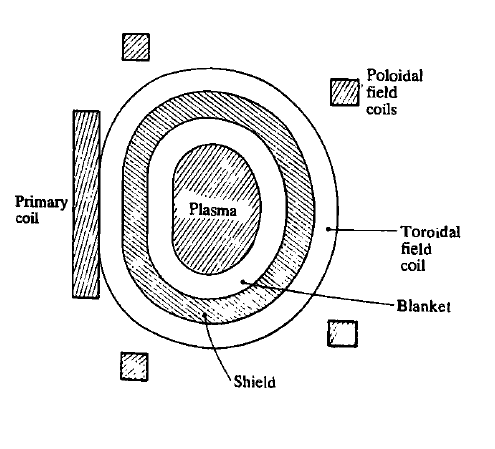
\includegraphics[width=0.4\textwidth]{Image/reactor.png}
        \caption{Structure of reactor}
        \label{fig:reactor}
\end{figure}

The blanket is used to capture neutron and convert the kinetic energy to heat in order to extract it. 

\chapter{Experiment aspect of Fusion}
\section{Density Pertubation}
From Section4.6 of \cite{Principle}, microwave transmission phase shift will tell us the information of the plasma density.

\begin{equation}
    \Delta \phi =\frac{\omega}{c}[1-(1-\frac{\omega_p^2}{\omega^2})^{1/2}]L
\end{equation}

Where $\omega_p=\sqrt{\frac{4\pi ne^2}{m}}$

\chapter{Appendix}
\section{Potential and Field}

Maxwell Equations

\begin{eqnarray}
\begin{aligned}
    \nabla \cdot \textbf{E}{}&=\frac{\rho}{\epsilon_0}\\
    \nabla \cdot \textbf{B} &= 0\\
    \nabla \times \textbf{E} &= -\frac{\partial \textbf{B}}{\partial t}\\
     \nabla \times \textbf{B} &= \mu_0\textbf{J}+\mu_0\epsilon_0 \frac{\partial \textbf{E}}{\partial t}\\
\end{aligned}
     \label{eq:Maxwell}
\end{eqnarray}

Using vector potential to present magnetic field with Lorentz gauge
\begin{eqnarray}
     \textbf{B}= \nabla \times \textbf{A}\\
     \textbf{E}=-\nabla \phi -\frac{\partial \textbf{A}}{\partial t}\\
     \nabla \cdot \textbf{A}+ \frac{1}{c^2}\frac{\partial \phi}{\partial t}=0
\end{eqnarray}

\section{Ohm's Law}

Ohm's Law

\begin{equation}
    \textbf{E}+\frac{1}{c}\textbf{V}\times \textbf{B}= \frac{1}{\sigma}\textbf{J}
\end{equation}

Since $\left(\frac{1}{c}\textbf{V}\times \textbf{B}
\right)_{||}< O^2$, then 

\begin{equation}
    E_{||} = \frac{1}{\sigma_{||}}J_{||} + O^2
\end{equation}

\section{Doppler shift}

\begin{equation}
f=\left(\frac{c \pm v_{\mathrm{r}}}{c \pm v_{\mathrm{s}}}\right) f_{0}
\end{equation}

For $v_r \ll c$ 

\section{Pressure tensor}
In section 3.2.5 of Principle of plasma physics by Krall \cite{Principle}.
\begin{equation}
    P_\alpha(\textbf{x},t)=\bar{n}_\alpha m_\alpha\int (\textbf{v}-\textbf{V}_\alpha)(v-\textbf{V}_\alpha)f_\alpha(\textbf{x},\textbf{v},t)d\textbf{v}
\end{equation}


\section{Magnetic pressure}

Magnetic pressure can be expressed as $P_{B}=\frac{B^{2}}{8 \pi}$


\section{Ballooning transformation}

Since the poloridal and toroidal angel $\theta \in (-\infty, \infty)$, for convenience. we define a function

\begin{equation}
z(\theta)=\sum_{l=-\infty}^{\infty} \bar{z}(\theta+2 \pi l)
\end{equation}

So all the function on the same location with but different winding times added together. 

\section{$(\phi,\zeta ,\chi)$}

$\phi$ is the radius-like coordinate, same $\phi$ means same magnetic surface. $\zeta$ is toroidal angle-like coordinate, $\chi$ is poloidal angle-like coordinate. \cite{Ballooning_transformation}

\section{MHD approximation}



\section{Gyro-average\label{sec:gyro}}

\subsection{Overview}
A great resource for gyro-average is the early paper of GENE\cite{merz} "Integrals for the field equations"

\begin{equation}
A(\vec{X}+\vec{r})=\sum_{k_{x}, k_{y}} A\left(k_{x}, k_{y}\right) e^{i \vec{k}_{\perp} \cdot(\vec{X}+\vec{r})}
\end{equation}
\begin{equation}
\begin{aligned}
    A(\textbf{x})
    {}&\longrightarrow< A(\textbf{X})>=A\left(k_{x}, k_{y}\right)J_0(k_\perp \rho_s)\\
    &\longrightarrow< A(\textbf{x})>=A\left(k_{x}, k_{y}\right)J_0^2(k_\perp \rho_s)\\
    &\longrightarrow A(\textbf{k})=A(\textbf{x})J_0(k_\perp \rho_s)
    \end{aligned}
\end{equation}


\subsection{Derivation}

For helix motion, we have

\begin{eqnarray}
    \Vec{x}= \rho_s cos(\omega t)\hat{x}+\rho_s sin(\omega t)\hat{y}+ x_{c} \hat{z}\\
    \omega =\frac{qB}{m}\\
    \rho_s=\frac{mv}{q_sB}
\end{eqnarray}

Where $x_{c}$ is the guiding center of the particle.

For any quantities that depends on the trajectory of charged particles will be taken average over gyro-radius. The following average method only works for $\frac{\omega}{\omega_g}\ll 1$ frequency of the of mode less than the gyro-frequency. The mode frequency is so slow that for a period of gyro-motion, the quantity of interest will stay constant.

The gyro-average of a scalar field can be written as

\begin{equation}
\begin{aligned}\langle A(X)\rangle &=\frac{1}{2 \pi} \int_{0}^{2 \pi} A(\vec{X}+\vec{r}) d \theta=\frac{1}{2 \pi} \int_{0}^{2 \pi} \sum_{k_{x}, k_{y}} A\left(k_{x}, k_{y}\right) e^{i \vec{k}_{\perp} \cdot(\vec{X}+\vec{r})} d \theta \\ 
&=\sum_{k_{x}, k_{y}} A\left(k_{x}, k_{y}\right) e^{i \vec{k}_{\perp} \cdot \vec{X}} \frac{1}{2 \pi} \int_{0}^{2 \pi} e^{i \vec{k}_{\perp} \cdot \vec{r}} d \theta \\
&=\sum_{k_{x}, k_{y}} A\left(k_{x}, k_{y}\right) e^{i \vec{k}_{\perp} \cdot \vec{X}} \frac{1}{2 \pi} \int_{0}^{2 \pi} e^{ik_{\perp} r cos\theta} d \theta \\
&=\sum_{k_{x}, k_{y}} A\left(k_{x}, k_{y}\right) e^{i \vec{k}_{\perp} \cdot \vec{X}} J_{0,s}(k_{\perp}\rho )\\
\end{aligned}
\label{eq:gyro_avg}
\end{equation}

Where $J_{0,s}(k_{\perp}\rho )=\frac{1}{2\pi} \int d \theta e^{ik_{\perp}\rho_s cos \theta}$. Therefore gyro-average introduces a $J_{0,s}(k_{\perp}\rho )$. Here is a plot of $J_0$ shown on Figure \ref{fig:J0}

\begin{figure}[h] \centering
        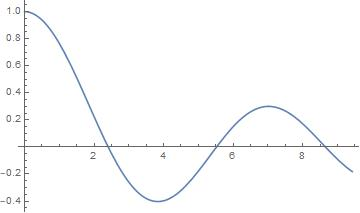
\includegraphics[width=0.5\textwidth]{Image/J0.jpg}
        \caption{Plot of Bessel function of first kind $J_0(x)$}
        \label{fig:J0}
    \end{figure}

From the guiding center to the real space is \cite{merz}

\begin{equation}
\begin{aligned}\langle\overline{A}(\vec{x}-\vec{r})\rangle &=\frac{1}{2 \pi} \int_{0}^{2 \pi} \frac{1}{2 \pi} \int_{0}^{2 \pi} A\left(\vec{x}-\vec{r}+\vec{r}^{\prime}\right) d \theta d \theta^{\prime} \\ &=\frac{1}{4 \pi^{2}} \int_{0}^{2 \pi} \int_{0}^{2 \pi} \sum_{k_{x}, k_{y}} A\left(k_{x}, k_{y}\right) e^{i \vec{k}_{\perp} \cdot\left(\vec{X}-\vec{r}+\vec{r}^{\prime}\right)} d \theta d \theta^{\prime} \\ &=\sum_{k_{x}, k_{y}} A\left(k_{x}, k_{y}\right) e^{i \vec{k}_{\perp} \cdot \vec{X}} J_{0}^{2}\left(\rho k_{\perp}\right) \end{aligned}
\end{equation}

For a velocity that is changing with frequency of gyro frequency, curvature drift velocity for instance, \cite{Vd} \cite{iter_scale}

\begin{equation}
    \begin{aligned}
        <\Tilde{v}^2_{\perp}>{}&=<v^2_{\perp}cos^2(\omega t)>\\
        &=\frac{\omega}{2\pi}\int^{\frac{2\pi}{\omega} }_{0}v^2_{\perp}cos^2(\omega t) dt\\
        &=\frac{1}{2} v^2_{\perp}
    \end{aligned}
\end{equation}

    
\section{Quasi-neutrality}

The assumption of quasi-neutrality is based on low oscillation frequency of the mode of interest compared with plasma frequency. 

\begin{equation}
    \frac{\omega}{\omega_p} \ll 1
\end{equation}

\section{Curl}
    For the Vector in the form of $\widetilde{\textbf{A}}=\textbf{A} e^{i\textbf{kx}-i\omega t}$. We can calcuate the curl as shown below. Where $A$ is a constant in terms of time and position. 
    \begin{eqnarray}
        \nabla \times (f\textbf{A}) = f \nabla \times \textbf{A} +(\nabla f)\times \textbf{A}\\
        \nabla \times (e^{i\textbf{kx}-i\omega t}\textbf{A}) = e^{i\textbf{kx}-i\omega t} \nabla \times \textbf{A} +(\nabla e^{i\textbf{kx}-i\omega t})\times \textbf{A}\\
        \nabla \times \widetilde{\textbf{A}}=  i\textbf{k} \times \widetilde{\textbf{A}}
    \end{eqnarray}
    Assuming $\textbf{A}=A\hat{z}, \textbf{k}=k\hat{y}$
    \begin{eqnarray}
    \begin{aligned}
        \textbf{B}e^{i\textbf{kx}-i\omega t}{}&= i\textbf{k}\times \widetilde{\textbf{A}}\\
        &=ik A e^{i\textbf{kx}-i\omega t}\hat{x}
        \label{eq:curl}
    \end{aligned}
    \end{eqnarray}
    
Based on Maxwell's equations:

\begin{eqnarray}
\begin{aligned}
    \nabla \textbf{E}{}&=\frac{\rho}{\epsilon_0}\\
    \nabla \textbf{B} &= 0\\
    \nabla \times \textbf{E} &= -\frac{\partial \textbf{B}}{\partial t}\\
     \nabla \times \textbf{B} &= \mu_0\textbf{J}+\mu_0\epsilon_0 \frac{\partial \textbf{E}}{\partial t}\\
\end{aligned}
     \label{eq:Maxwell}
\end{eqnarray}
Using vector potential to present magnetic field with Lorentz gauge
\begin{eqnarray}
     \textbf{B}= \nabla \times \textbf{A}\\
     \textbf{E}=-\nabla \phi -\frac{\partial \textbf{A}}{\partial t}\\
     \nabla \textbf{A}+ \frac{1}{c^2}\frac{\partial \phi}{\partial t}=0
\end{eqnarray}

Therefore we can express magnetic field and electric field as following way:
\begin{eqnarray}
     \textbf{B}= i\textbf{k}\times \textbf{A}\\
     \textbf{E} = -i\textbf{k} \phi +i\omega \textbf{A}
     \label{eq:E-A}
\end{eqnarray}

\begin{eqnarray}
     \nabla \times (\nabla \times \textbf{A})=\nabla (\nabla \textbf{A}) -\nabla^2 \textbf{A}\\
     \nabla^2 \textbf{A}=\frac{\omega^2}{c^2} \textbf{A}-\frac{4\pi}{c} \textbf{J}\\
     (k^2-\frac{\omega^2}{c^2})A_{||}=-\frac{4\pi}{c}J_{||}\\
    \nabla \times (\nabla \times \textbf{A})=\frac{4\pi}{c} \textbf{J}
\end{eqnarray}

\section{Common Quantities}

\subsection{Toroidal coordinates}
For the simplicity, plasma physicists use toroidal coordinates. We define the following quantities.

Here is the coordinate $(r, \phi, \theta)$. 

\begin{eqnarray}
\begin{aligned}
    R=major\ radius\\
    r= minor\ radius\\
    \zeta=\phi= toroidal\ angle\\
    \theta = poroidal\ angle
\end{aligned}
\end{eqnarray}

\subsection{Shafranov shift}

\begin{eqnarray}
     \begin{aligned}
      r’{}&=R_0+\Delta(r)-r cos\alpha\\
      \theta’&=\zeta\\
      z’&=r sin\alpha=r sin(\theta+\delta)
     \end{aligned}
\end{eqnarray}

\subsection{Flux coordinates}

Flux coordinates can be express in the following fashion: $(\psi, \chi, \zeta)$

Where $\psi$ is magentic flux, which is defined as 

\begin{eqnarray}
\begin{aligned}
   \phi_p{}&=\int \textbf{B}_Td\textbf{s}\\
   \phi_T&=\int \textbf{B}_Pd\textbf{s}\\
\end{aligned}
\end{eqnarray}

Since magnetic field is pointing at the same direction with varying radius, The magnitude of magnetic flux is monotonically increasing, that means one can map the magnetic flux to radius is a one-to-one manner. 

\subsection{Wave number}
The wave number in GENE refers to the magnetic field, which can be considered as operator 

\begin{eqnarray}
\begin{aligned}
    k_{||}{}&=-i\nabla_{||}\\
    &=-i\textbf{b}\cdot \nabla \\
    &=-i\frac{B_z}{B_0}(\hat{e}_{\zeta}+\frac{r}{qR}\hat{e}_{\theta})\cdot(\hat{e}_{r}\frac{\partial}{\partial r}+\hat{e}_{\theta}\frac{1}{r}\frac{\partial}{\partial \theta}+\frac{1}{R}\hat{e}_{\zeta}\frac{\partial}{\partial \zeta})\\
    &=-i\frac{B_z}{B_0}(\frac{1}{qR}\frac{\partial}{\partial \theta }+\frac{1}{R}\frac{\partial}{\partial \zeta})\\
    &= -i \frac{B_z}{B_0}\frac{1}{qR}(\frac{\partial}{\partial \theta }+q\frac{\partial}{\partial \zeta})
\end{aligned}
\end{eqnarray}

If we apply this operator to a wave function $\phi=\phi(r)e^{im\theta -in \zeta }\sum_l e^{i l\theta}$
For slab geometry, $l=0$, therefore, we have the following equation,

\begin{eqnarray}
\phi=e^{im\theta -in \zeta }\\
k_{||}\phi = \frac{B_z}{B_0}\frac{1}{qR}(m - qn)\phi
\end{eqnarray}

From $k_{||}$, one can get $k_{\perp}$ 

\begin{eqnarray}
\begin{aligned}
\nabla_{\perp}{}&=\nabla -\nabla_{||}\\
%&=(\hat{b}\nabla)\hat{b}-(\hat{b} \cdot \hat{b})\nabla\\
%&=\hat{b}\times(\hat{b}\times \nabla)\\
&=\hat{e}_{r}\frac{\partial}{\partial r}+\hat{e}_{\theta}\frac{1}{r}\frac{\partial}{\partial \theta}-\frac{1}{qR}\hat{e}_{\zeta}\frac{\partial}{\partial \theta}
\end{aligned}
\end{eqnarray}

Since $\frac{r}{R}\ll 1$, then it is valid to drop the third term. Therefore, we have:

\begin{eqnarray}
\nabla_{\perp}=\hat{e}_{r}\frac{\partial}{\partial r}+\hat{e}_{\theta}\frac{1}{r}\frac{\partial}{\partial \theta}
\end{eqnarray}

Then we have (In GENE coordinates)

\begin{eqnarray}
\begin{aligned}
k_{x}{}&=-i\frac{\partial}{\partial r}\\
k_{y}&=-i\frac{1}{r}\frac{\partial}{\partial \theta}\\
k_z&=k_{||}=-i \frac{1}{qR}(\frac{\partial}{\partial \theta }+q\frac{\partial}{\partial \zeta})
\end{aligned}
\end{eqnarray}

Plug $k_x$ and $k_y$ into $\phi=e^{im\theta -in \zeta }$\\

\begin{eqnarray}
\begin{aligned}
k_{x}\phi{}&=-i\frac{\partial}{\partial r}\phi\\
k_{y}\phi&=\frac{m}{r}\phi\\
k_{z}\phi&=k_{||}\phi= \frac{m-nq}{qR}\phi
\label{eq:k_slab}
\end{aligned}
\end{eqnarray}

For the most cases, $\frac{r}{\rho_s}=500$. Where $\rho_s$ is the gyro-radii. So if $k_y\rho_s$ is smaller than 0.02, then we are in region that m is in the order of 10. then $k_y\rho_s$ is will be less continuous since m has to be a integer. 

\subsection{Bootstrap current}

The Bootstrap current is induced by $\frac{\nabla p \times B_p}{B}$ where $B_p$ is the poloridal magnetic field. From the Wesson's book Tokamaks \cite{Tokamaks}


\begin{equation}
j_{\mathrm{b}}=-\frac{\varepsilon^{1 / 2} n}{B_{\theta}}\left[2.44\left(T_{\mathrm{e}}+T_{\mathrm{i}}\right) \frac{1}{n} \frac{\mathrm{d} n}{\mathrm{d} r}+0.69 \frac{\mathrm{d} T_{\mathrm{e}}}{\mathrm{d} r}-0.42 \frac{\mathrm{d} T_{\mathrm{i}}}{\mathrm{d} r}\right]
\end{equation}

The bootstrap current will induce magnetic field that is opposite the $B_p$. That is the the reason why the pedestal region where the pressure gradient is high. The magnetic shear is small. As the the Figure\ref{fig:j_bs} shows. 

\begin{figure}[h] \centering
        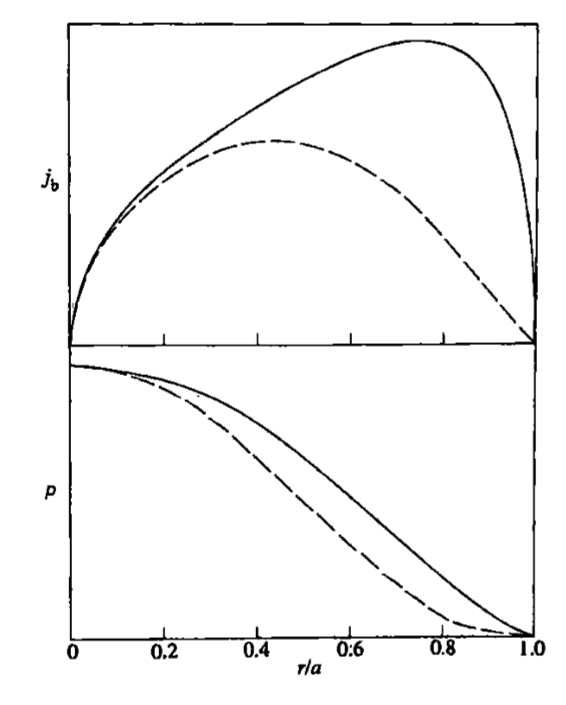
\includegraphics[width=1\textwidth]{Image/BS_current.png}
        \caption{Bootstrap current distribution in radius}
        \label{fig:j_bs}
\end{figure}


The origin of the bootstrap current comes from the the idea that bootstrap current will be one of the component that will make the fusion devices self-sustainable. 


\subsection{safety factor and rational surface}

\subsubsection{Safety factor}

Safety factor can be understood as "twistiness of the magnetic field", which can be expressed as 

\begin{eqnarray}
q=\frac{B_{tor}}{2\pi R} (\frac{B_{por}}{2\pi r})^{-1}
\end{eqnarray}

One can also think that $\frac{2\pi}{q}$ is how much the magnetic field have turned after a turn toroidally or $q=\frac{d \phi}{d \theta}$

\subsubsection{Rational surface}

Rational surface is the surface when q is rational e.g. q can be expressed as  $q=\frac{m}{n}$.That means it takes n turns toroidally, and m turns poroidally to get back to the original spot.  n is the toroidal mode number, m is the poloidal mode number




\section{Dedye shielding \label{sec:debye}\cite{Chen}}

From 1-D Poisson's Equation:

\begin{eqnarray}
\frac{\partial^2 \phi}{\partial x^2} =-4\pi e(n_i-n_e)
\end{eqnarray}

With the potential of $q\phi$ and the kinetic energy $\frac{1}{2}mv^2$, we have the distribution function as following:

\begin{equation}
f(v)=A \exp \left[-\left(\frac{1}{2} m v^{2}+q \phi\right) / T_{e}\right]
\end{equation}

The distance of a ion to a ion is much further than electron, i.e. $r_i\gg r_e$. $f_i \approx A\exp[-\frac{m_iv^2}{2T_e}]$

With the relationship of density and distribution function: 

\begin{eqnarray}
 n_s=\int f(v) dv\\
 n_i=n_0\\
 n_e=n_0 \exp (e\phi/T_e)\\
 \rho_{tot}=-e(n_i-n_e)=en_0[\exp (e\phi/T_e)-1]\label{eq:neutral}
\end{eqnarray}


We can expand the distribution function in terms of $\frac{e\phi}{T_e}$ if $\frac{e\phi}{T_e}\ll 1$

\begin{eqnarray}
 \nabla^2 \phi = -\rho_{tot}\\
 \frac{\partial^2 \phi}{\partial x^2}=4\pi en_0[(e\phi/T_e)+\frac{1}{2}(e\phi/T_e)^2+...]
\end{eqnarray}

Take the first order of the Taylor Expansion, can solve this differential equation with ease,

\begin{equation}
    \phi=\phi_0e^{\pm x\sqrt{\frac{4\pi n_0e^2}{T_e}}}
\end{equation}

For the sake of convergence, we left with only one solution, 

\begin{equation}
    \phi=\phi_0e^{- x\sqrt{\frac{4\pi n_0e^2}{T_e}}}
\end{equation}

Define Debye length $\lambda_D=\sqrt{\frac{T_e}{4\pi n_0e^2}}$, then we have

\begin{equation}
     \phi=\phi_0e^{-x/\lambda_D}
\end{equation}

The physical understanding of Debye length is that beyond which length, charged particle will not experience the significant amount of electric field. 

Quasi neutrality can be implied from the derivation above, From Equation \ref{eq:neutral}, we can see that $\rho_{tot} \approx 0$ which is quasi neutral. Therefore we can will have the following conclusion 

\begin{eqnarray}
 \frac{e\phi}{T_e}\ll 1 \Longrightarrow \rho_{tot} \approx 0
\end{eqnarray}

$1_{st}$ order adiabatic perturbation can be implied from it as well, the distribution function can be expanded

\begin{equation}
    f_e=Ae^{-\frac{mv^2}{2T}}[1+(\frac{q\phi}{T_e})+\frac{1}{2}(\frac{q\phi}{T_e})^2+...]
\end{equation}

The first term is $0_{th}$ order - Maxwellian distribution, second term is the $1_{st}$ order adiabatic perturbed term.

\subsection{Adiabatic perturbed term}

Let's assume we have the magnetic term in the adiabatic perturbed term.Similar to the Debye shielding, we can use the Hamiltonian to derive the adiabatic perturbed term. 

\begin{equation}
\begin{aligned}
    f{}&=F_0\left(1+\frac{q_s\textbf{v}\cdot \textbf{A}}{cT_s}-\frac{q_s\phi}{T_s} \right)+h_s\\
    &=F_0+\delta f
\end{aligned}
\end{equation}

Where $F_0$ is the Maxwellian distribution, $F_0\left(\frac{q_s\textbf{v}\cdot \textbf{A}}{cT_s}-\frac{q_s\phi}{T_s} \right)$ is adiabatic perturbed term, $h_s$ is the non-adiabatic perturbed term

Plug into Equation\ref{eq:temp23}, 

\begin{equation}
\begin{aligned}
    (\omega -\omega_D 
    - k_{||}v_{||})\left[F_0\left(\frac{q_sA_{||}v_{||}}{cT_s}-\frac{q_s\phi}{T_s} \right)+h_s\right]
    +\\
    \left[\omega_{*}^{tot}\frac{q_s\phi}{T_s}+
    (\omega-\omega^{tot}_*) \frac{q_s A_{||}v_{||}}{cT_s}-(k_{||}v_{||}+\omega_D)\frac{q_s\phi}{T_s}\right]F_0
    =i\left(\frac{\partial f}{\partial t}\right)_{\mathrm{coll}}
\end{aligned}
\end{equation}

After some algebra, we are left with

\begin{equation}
     (\omega -\omega_D 
    - k_{||}v_{||})h_s 
    -(\omega -\omega_*^{tot})\frac{q_s\phi}{T_s}F_0+(2\omega -\omega^{tot}-\omega_D-k_{||}v_{||})\frac{q_sA_{||}v_{||}}{cT_s}F_0
    =i\left(\frac{\partial f}{\partial t}\right)_{\mathrm{coll}}
\end{equation}

If we assume $i\left(\frac{\partial f}{\partial t}\right)_{\mathrm{coll}} = -i\nu(h_s) h_s$, then we can obtain the following expression

\begin{equation}
    h_s 
    =\frac{\omega -\omega_*^{tot} 
    }{\omega -\omega_D 
    - k_{||}v_{||}+i\nu(h_s)}\left(\frac{q_s\phi}{T_s}-\frac{q_sA_{||}v_{||}}{cT_s}\right)F_0 - \frac{q_sA_{||}v_{||}}{cT_s}F_0
    \label{eq:linear2}
\end{equation}

When it is effectively 

\begin{equation}
    \delta f =-\frac{q_s\phi}{T_s}F_0+h_s
    \label{eq:adiabatic}
\end{equation}

Where $
    h_s 
    =\frac{\omega -\omega_*^{tot} 
    }{\omega -\omega_D 
    - k_{||}v_{||}+i\nu(h_s)}\left(\frac{q_s\phi}{T_s}-\frac{q_sA_{||}v_{||}}{cT_s}\right)F_0
$

\subsection{$Delta$(Delta)}

From \cite{tearing_parity} Appendix, the explanation was given for $Delta$. 



\section{Maxwellian distribution}

The origin of Maxwellian distribution ($\sqrt{\frac{m}{2\pi  T}}e^{-\frac{mv^2}{2T}}$)can be traced back to the Boltzmann distribution ($p\propto e^{-\frac{\epsilon}{T}}$) microscopic statistical mechanics. However, one can derive Maxwellian distribution from Boltzmann Equation with no force. 

From collisional plasma physics point of view, the\textbf{ H theorem} will be the answer to the equilibrium distribution being Maxwellian. 

\begin{equation}
    \frac{\partial f}{\partial t} +\Vec{v} \nabla f +\Vec{F}\frac{\partial f}{\partial \epsilon}=(\frac{\partial f}{\partial t})_{coll}
\end{equation}

For the future reference, we can examine it by plugging in the Maxwellian equation$F_0=\sqrt{\frac{m}{2\pi T}}e^{-\frac{mv^2}{2T}}$

\begin{eqnarray}
 \frac{\partial F_0}{\partial t}=0\\
 \frac{\partial F_0}{\partial \epsilon}=\frac{1}{T}F_0\\
 \nabla F_0 = \left[\frac{\nabla n_0}{n_0}+(\frac{3}{2}-\frac{mv^2}{2T})\frac{\nabla T_0}{T_0}\right]F_0\\
 \vec{F}=q(\vec{E}+\vec{v}\times \vec{B})\\
 \vec{v}_{||}\nabla F_0=0
\end{eqnarray}

Where force is negligible. The density and temperature change along the field line is small. 

\section{Gaussian Unit \label{sec:gauss}}

Maxwell's Equations

\begin{equation}
\begin{array}{l}
{\nabla \cdot \mathbf{E}=4 \pi \rho} \\ 
{\nabla \cdot \mathbf{B}=0} \\ 
{\nabla \times \textbf{E} = -\frac{1}{c}\frac{\partial \textbf{B}}{\partial t}}\\
{\nabla \times \mathbf{B}=\frac{4 \pi}{c} \mathbf{J}+\frac{1}{c} \frac{\partial \mathbf{E}}{\partial t}}
\end{array}
\end{equation}

And $k_B=1$

Here are some good quantities

\begin{eqnarray}
 v_E=\frac{E_{SI}}{B_{SI}}=\frac{1}{c}\frac{E_G}{B_G}
\end{eqnarray}

Here is the conversion from SI unit to Gauss Unit\cite{Handbook}

\begin{equation}
\begin{array}{lll}{\epsilon_{0} \mapsto 1 /(4 \pi)} & {\mu_{0} \mapsto 4 \pi / c^{2}} & {B \mapsto B / c} \\ {\chi_{E} \mapsto 4 \pi \chi_{E}} & {\chi_{H} \mapsto 4 \pi \chi_{H}} & {H \mapsto c H /(4 \pi)} \\ {A \mapsto A / c} & {M \mapsto c M} & {D \mapsto D /(4 \pi)}\end{array}
\end{equation}

A good place to check it Wikipedia 

\begin{verbatim}
    https://en.wikipedia.org/wiki/Gaussian_units
\end{verbatim}

\section{Ordering}

$R_c$ is the curvature of the device which is in the order of the major radius of the device. 

$r_g$ is the gyro-radius.Commonly, magnetic field is the order of 5T. 

\begin{equation}
    \begin{aligned}
    R_c ~ 5m
    r_g=\frac{mv_{\perp}}{qB} ~ 1cm
    \end{aligned}
\end{equation}

With ordering law of the 

\begin{equation}
\begin{aligned}
v_D{}&=\left(v_{ \|}^{2}+\frac{1}{2} v_{\perp}^{2}\right) \frac{m}{q} \frac{\mathbf{R}_{c} \times \mathbf{B}}{R_{c}^{2} B^{2}}\\
\frac{v_D}{v_{||}}&\approx \frac{v_{||} m}{R_cB_0q}\\
\frac{v_D}{v_{||}}&\approx \frac{v_{||}}{v_{\perp}}\frac{r_g}{R_c}
\label{eq:vD}
\end{aligned}
\end{equation}

\section{Collision\cite{coll}}\label{sec:coll}

Define $\hat{c}=\frac{\textbf{g}_f-\textbf{g}_i}{|\textbf{g}_f-\textbf{g}_i|}$, where $\textbf{g}=\textbf{v}_1-\textbf{v}_2$. f stand for final, i stands for initial. 

\begin{equation}
    \hat{c}=cos\left(\frac{\chi}{2}\right)(cos\phi \hat{x}_i+sin\phi \hat{y}_i)-sin\left(\frac{\chi}{2}\right)\frac{\textbf{g}_i}{g_i}
\end{equation}

As figure \ref{fig:coll1} shown, $\chi$ is the angle between $\textbf{g}_i$ and $\textbf{g}_f$

\begin{figure}[h] \centering
        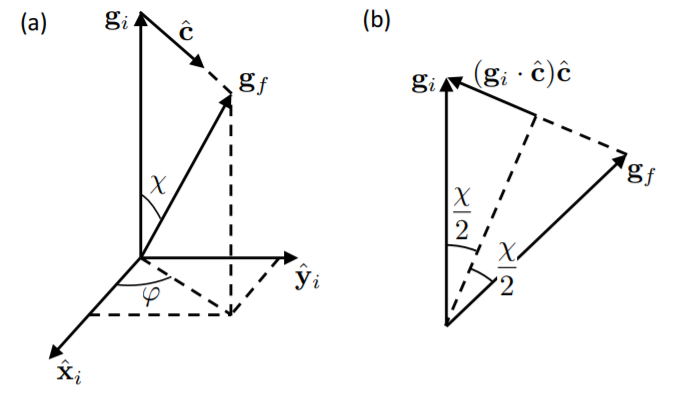
\includegraphics[width=1\textwidth]{Image/coll1.PNG}
        \caption{Diagram of the setup of binary collision}
        \label{fig:coll1}
\end{figure}

We define the following relation

\begin{equation}
\mathbf{g}_{f}=\underline{\mathbf{g}}_{i} \equiv(\mathbf{I}-2 \hat{\mathbf{c}} \hat{\mathbf{c}}) \cdot \mathbf{g}_{i}
\end{equation}

Then we have

\begin{equation}
\mathbf{g}_{i}=\mathbf{g}_{f} \equiv(\mathbf{I}-2 \hat{\mathbf{c}} \hat{\mathbf{c}}) \cdot \mathbf{g}_{f}
\end{equation}

\begin{equation}
\underline{\underline{g}_{i}}=(\mathbf{I}-2 \hat{\mathbf{c}} \hat{\mathbf{c}}) \cdot(\mathbf{I}-2 \hat{\mathbf{c}} \hat{\mathbf{c}}) \cdot \mathbf{g}_{i}=[\mathbf{I}-4 \hat{\mathbf{c}} \hat{\mathbf{c}}+4(\hat{\mathbf{c}} \cdot \hat{\mathbf{c}}) \hat{\mathbf{c}} \hat{\mathbf{c}}] \cdot \mathbf{g}_{i}=\mathbf{g}_{i}
\end{equation}

Define $Q=\mathbf{I}-2 \hat{\mathbf{c}} \hat{\mathbf{c}}$

Here is heuristic derivation from BBGKY approach \cite{coll2}. 

\begin{equation}
\begin{array}{l}{\int X(\mathbf{r}, \mathbf{v}, t) C_{s s^{\prime}}\left[f_{s}, f_{s^{\prime}}\right](\mathbf{r}, \mathbf{v}, t) \mathrm{d}^{3} v=} \\ {\int \mathrm{d}^{3} v f_{s}(\mathbf{v}) \int \mathrm{d}^{3} v^{\prime} f_{s^{\prime}}\left(\mathbf{v}^{\prime}\right) \int_{0}^{2 \pi} \mathrm{d} \varphi \int_{0}^{\pi} \mathrm{d} \chi g \sigma_{s s^{\prime}}(g, \chi) \sin \chi[X(\underline{\mathbf{v}})-X(\mathbf{v})]}\end{array}
\end{equation}

Where $X$ is any function, $\sigma$ is cross section $\sigma_{s s^{\prime}}=\frac{\rho}{\sin \chi}\left|\frac{\partial \rho}{\partial \chi}\right|$.

\subsection{Coulomb collisions}

With potential 

\begin{equation}
V(r)=\frac{Z_{s} Z_{s^{\prime}} e^{2}}{4 \pi \epsilon_{0} r}
\end{equation}

Apply conservation of energy and angular momentum

\begin{equation}
\begin{aligned} \frac{\mathrm{d} r}{\mathrm{d} \theta}=\frac{\mathrm{d} r / \mathrm{d} t}{\mathrm{d} \theta / \mathrm{d} t} &=\pm \frac{r^{2}}{\rho} \sqrt{1-\frac{2 b_{s s^{\prime}}}{r}-\frac{\rho^{2}}{r^{2}}}
\end{aligned}
\end{equation}

Where $b_{s s^{\prime}}=\frac{Z_{s} Z_{s}^{\prime} e^{2}}{4 \pi \epsilon_{0} \mu_{s s^{\prime}}^{\prime} g^{2}}$

After integration, we have Rutherford cross section

\begin{equation}
\sigma_{s s^{\prime}}=\frac{b_{s s^{\prime}}^{2}}{4 \sin ^{4}(\chi / 2)}
\end{equation}

\subsection{Fokker-Planck collision operator}

If we assume $\chi \ll 1$ then we have

\begin{equation}
\sigma_{s s^{\prime}} \simeq \frac{4 b_{s s^{\prime}}^{2}}{\chi^{4}}
\end{equation}

We ended up with the Landau form of Fokker-Planck
collision operator

\begin{equation}
C_{s s^{\prime}}\left[f_{s}, f_{s^{\prime}}\right]=\frac{\gamma_{s s^{\prime}}}{m_{s}} \nabla_{v} \cdot\left\{\int \nabla_{g} \nabla_{g} g \cdot\left[\frac{f_{s^{\prime}}\left(\mathbf{v}^{\prime}\right)}{m_{s}} \nabla_{v} f_{s}(\mathbf{v})-\frac{f_{s}(\mathbf{v})}{m_{s^{\prime}}} \nabla_{v^{\prime}} f_{s^{\prime}}\left(\mathbf{v}^{\prime}\right)\right] \mathrm{d}^{3} v^{\prime}\right\}
\end{equation}

With H-theorm

\begin{equation}
\dot{\sigma}_{s s^{\prime}}+\dot{\sigma}_{s^{\prime} s} \geqslant 0
\end{equation}

Where $\dot{\sigma}_{s s^{\prime}}=-\int \ln f_{s}(\mathbf{r}, \mathbf{v}, t) C_{s s^{\prime}}\left[f_{s}, f_{s^{\prime}}\right](\mathbf{r}, \mathbf{v}, t) \mathrm{d}^{3} v$
and $\dot{\sigma}_{s s^{\prime}}+\dot{\sigma}_{s^{\prime} s}$ is equal to zero only when both $f_{s}$ and $f_{s^{\prime}}$ are Maxwellians with the same
average velocity $\mathbf{u}$ and temperature $T$.

The H-theorem of the Fokker-Planck collision operator implies that the only solutions
to the system of equations 

\begin{equation}
\begin{array}{l}{C_{s s^{\prime}}\left[f_{s}, f_{s^{\prime}}\right]=0} \\ {C_{s^{\prime} s}\left[f_{s^{\prime}}, f_{s}\right]=0}\end{array}
\end{equation}

are the Maxwellian

\subsection{Krook Collation Operator}

Let's start from lineariezed Fokker Plank collision operator between electron and ion: Equation 24 in \cite{MTM_RH}, 

\begin{equation}
C_{e i}^{l}=\frac{3 \sqrt{\pi}}{4 \tau} v_{t_{e}}^{3}\left(\frac{1}{2 v^{3}} \frac{\partial}{\partial \zeta}\left(1-\zeta^{2}\right) \frac{\partial f_{1 e}}{\partial \zeta}+\frac{2 V_{|| i} \zeta}{v_{t_{e}}^{2} v^{2}} f_{M_{e}}\right)
\label{eq:linear_coll}
\end{equation}

Where $\zeta \equiv v_{n} / v$ is the cosine of the pitch angle. 

Recall Legendre differential equation

\begin{equation}
\frac{d}{d x}\left[\left(1-x^{2}\right) \frac{d y}{d x}\right]+l(l+1) y=0
\label{eq:legendre_diff}
\end{equation}

whose solutions are Legendre polynomials

\begin{equation}
\begin{array}{l}{P_{0}(x)=1} \\ {P_{1}(x)=x} \\ {P_{2}(x)=\frac{1}{2}\left(3 x^{2}-1\right)} \\ {P_{3}(x)=\frac{1}{2}\left(5 x^{3}-3 x\right)} \\ {P_{4}(x)=\frac{1}{8}\left(35 x^{4}-30 x^{2}+3\right)} \\ {P_{5}(x)=\frac{1}{8}\left(63 x^{5}-70 x^{3}+15 x\right)} \\ {P_{6}(x)=\frac{1}{16}\left(231 x^{6}-315 x^{4}+105 x^{2}-5\right)}\end{array}
\label{eq:legendre_poly}
\end{equation}

If the perturbed term can be expressed in terms of the eigenfunctions of Legendre differential equation, such that $f_{1e}=\sum a_ly_l(\zeta)$, then the first term of Equation\ref{eq:linear_coll} can be simplified

\begin{equation}
C_{e i}^{l}=\frac{3 \sqrt{\pi}}{4 \tau} v_{t_{e}}^{3}\left(-\frac{1}{2 v^{3}} 
\sum l(l+1)a_ly_l(\zeta)
+\frac{2 V_{|| i} \zeta}{v_{t_{e}}^{2} v^{2}} f_{M_{e}}\right)
\end{equation}

we just take the factor in front of the 
\begin{eqnarray}
     \nu=C_{e i}^{l}\approx \frac{\nu_0\cdot v_{th}^3}{v^3}
\end{eqnarray}

\subsection{Derivation}

The derivation is rather "hand wavy". Please check if it work for your parameters. 

For adiabatic perturbed term $\frac{q_s\phi}{T_s}F_{0,s}$, which is not a function of $\zeta$, it will not appear on the collisional term. 

Recall the non-adiabatic perturbed term from Equation \ref{eq:linear_tot}

\begin{equation}
h_{e}=\frac{\omega-\omega_{* e}^{t o t}}{\omega-\omega_{D, e}-k_{ \|, e} v_{ \|}-i \nu\left[h_{e}\right]}\left(\frac{q_{e} \phi}{T_{e}}-\frac{q_{e} A_{ \|} v_{ \|}}{c T_{e}}\right) J_{0}^{2}\left(k_{\perp} \rho_{e}\right) F_{0, e}
\end{equation}

Can assume the $\nu$ is not a function of $\zeta$. 

For spherical coordinate $\zeta =cos\theat =\frac{v_{||}}{v}$, thus $v_\perp=v\sqrt{1-\zeta^2}$ for $\omega_{*}^{T o t}=\omega_{* n}+\left(-\frac{3}{2}+\frac{v_{\perp}^{2}+v_{ \|}^{2}}{2 v_{t h}^{2}}\right) \omega_{* T}$, it does not depend on $\zeta$, and recall $\omega_D=-k_{y} \frac{v_{\perp}^{2} / 2+v_{ \|}^{2}}{R_{c} \Omega}$ and $\Omega=\frac{m v_\perp c}{q B}$. 

\begin{equation}
h_{s}=\frac{\alpha}{\beta+
\gamma
 \frac{1+\zeta^2}{\sqrt{1-\zeta^2}}
-\eta\zeta}
\left(\frac{q_{e} \phi}{T_{e}}-\frac{q_{e} A_{ \|} v\zeta}{c T_{e}}\right) J_{0}^{2}\left(\kappa \zeta \right) F_{0, e}
\end{equation}

Where $\alpha=\omega-\omega_{* e}^{t o t}$, $\beta=\omega - i\nu$, $\gamma=\frac{k_yvqB}{2R_c mc} $, $\eta=k_{||,e}v$, $\kappa = \frac{k_\perp m_e v}{q_eB}$

For the sake of numberial calculation, we assume $\alpha=\beta=1$, $\gamma=\eta=\kappa=0.1$

Since Legendre polynomial is normalized, 

\begin{equation}
    a_n=\int^{1}_{-1} d\zeta f(\zeta) P_n(\zeta)
\end{equation}

For Electrostatic term, We have $a_0=1.66972$, $a_1=0.0389354$, $a_2=-0.0815086$, $a_3=-0.00695478$ (Check the mathematica code "coll.nb"), So the $0_{th}$ order is dominating. 

For Electromagnetic term, We have $a_0=0.0389354$, $a_1=0.502235$, $a_2=0.0114013$, $a_3=-0.0494179$ (Check the mathematica code "coll.nb"), So the $1_{st}$ order is dominating. 

Let's take the dominated terms to have a further investigation. 

\begin{equation}
    h_s=-1.66972\frac{e\phi}{T_e} f_1(v)+0.502235\frac{eA_{||}v}{cT_e}\zeta
\end{equation}

Where $f_1$ is a function that is depend on velocity and contains Maxwellian distribution. 

Plug it into the linearized collision operator 

$C_{e i}^{l}=\frac{3 \sqrt{\pi}}{4 \tau} v_{t_{e}}^{3}\left(-\frac{1}{2 v^{3}} \sum l(l+1) a_{l} y_{l}(x)+\frac{2 V_{|| i} \zeta}{v_{t_{e}}^{2} v^{2}} f_{M_{e}}\right)$,

\begin{equation}
C_{e i}^{l}\approx
\frac{3 \sqrt{\pi}}{4 \tau} v_{t_{e}}^{3}\left(-\frac{1}{2 v^{3}} 1.00447 \zeta f_1(v)+\frac{2 V_{|| i} \zeta}{v_{t_{e}}^{2} v^{2}} F_{0,e}\right)
\end{equation}

Since the pitch angle is close to 0, so $\zeta \approx 1$

\begin{equation}
C_{e i}^{l}\approx
\frac{3 \sqrt{\pi}}{4 \tau} v_{t_{e}}^{3}\left(-\frac{1}{2 v^{3}} 1.00447 f_1(v)+\frac{2 V_{|| i} }{v_{t_{e}}^{2} v^{2}} F_{0,e}\right)
\end{equation}

Since $\frac{v_i}{v_e}\ll1$, the second term can be neglected. 

Therefore
\begin{equation}
C_{e i}^{l}\approx-\nu_0
 \frac{v_{t_{e}}^{3}}{v^{3}} h_s
\end{equation}

Where $\nu_0
=
\frac{3 \sqrt{\pi}}{4 \tau}
$

\section{Alfvén wave}

From Chen's book \cite{}

\section{Formula}

\subsection{Fluid dynamics}

Bernoulli's Equation

\begin{equation}
p+\frac{1}{2} \rho V^{2}+\rho g h=\text {constant }
\end{equation}

\subsection{Statistical mechanics}

Adiabatic process
\begin{equation}
    pV^{\gamma}=constant
\end{equation}
Where $\gamma=(d+2)/d$

\section{Terminology}

ELM: edge located modes

Low field side: Outboard
High field side: Inboard


From s alpha geometry

\begin{equation}
 -\pi k_y \hat{s} < k_x< \pi k_y \hat{s}
\end{equation}





\medskip
 
\printbibliography

\end{document}
